\begin{center}
\begin{tabular}{| c | c | c | c | c | c | c | c | c | c | c | c | c | c |}
\hline
element & H$_2$NNH$_2$ & HNNH & N & N$_2$ & N$_2$H & N$_2$H$_2$ & N$_2$H$_3$ & NH & NH$_2$ & NH$_3$ & formation energy\\
\hline

Os & 0.61 & 0.39 & -0.7 & -1.17 & -0.15 & -0.36 & 0.06 & 0.06 & -1.26 & -1.29 & 6.31 \\
Pt &  & 2.16 & 2.77 & 0.26 & 1.78 & 2.06 & 1.44 & 1.69 & 0.08 & -0.09 & 6.86 \\
Cu & 1.33 & 2.07 & 4.51 & 0.18 & 2.33 & 2.4 & 1.65 & 3.41 & 0.95 & -0.45 &  \\
Tc & 1.03 & 0.95 & -0.87 & -0.65 & 0.06 & 0.27 & 0.65 & 0.52 & -0.69 & -0.92 & 4.58 \\
Y & 1.01 & 1.69 & 2.72 & 0.02 &  & 2.0 & 1.34 & 2.58 & 0.02 & -0.77 & -1.38 \\
Zr & 1.23 & 1.39 & 1.71 & -0.01 & 1.07 & 0.74 & 0.35 & 0.16 & -1.09 & -0.88 & -0.51 \\
Ag & 1.44 & 2.33 & 5.3 & 0.24 & 2.62 & 2.65 & 2.04 & 3.83 & 1.29 & -0.18 & 7.28 \\
Pd & 1.53 & 2.12 & 3.55 & 0.23 & 2.0 & 2.25 & 1.67 & 2.5 & 0.44 & -0.22 & 6.08 \\
Cr & 1.28 & 1.21 & -0.44 &  & 0.12 &  & -0.73 & 0.55 & -0.68 & -0.67 & 3.94 \\
Au & 1.68 & 2.36 & 4.05 & 0.25 & 2.54 &  & 2.15 & 2.95 & 0.92 & -0.08 & 8.18 \\
V & 1.43 & 1.5 & -0.33 & 0.04 & 0.82 & 0.38 & 0.55 & 0.17 & -0.86 & -1.03 & 2.48 \\
Hf & 1.21 & 1.32 & 1.59 & -0.02 & 0.97 & 0.6 & 0.2 & 0.02 & -1.26 & -0.95 & -0.92 \\
Co & 1.14 & 1.53 & 2.34 & 0.12 & 1.04 & 1.05 & 0.78 & 1.82 & -0.57 & -0.72 & 4.49 \\
Ir & 0.82 & 0.74 & 1.03 & -0.7 & 0.26 & 0.19 & -0.01 & 0.54 & -1.34 & -1.2 & 7.07 \\
Ta & 1.1 & 0.31 & -0.99 & -0.13 & 0.42 & -0.32 & -0.22 & -0.95 & -1.69 & -0.85 & 1.69 \\
Ti & 1.42 & 1.64 & 1.73 & 0.11 & 1.27 & 0.85 & 0.61 & 0.37 & -0.82 & -0.6 & 0.0 \\
Nb & 1.23 & 0.43 & -1.04 & -0.23 & 0.35 & -0.36 & -0.04 & -0.84 & -1.52 & -0.86 & 1.5 \\
Rh & 1.16 & 1.3 & 1.86 & -0.16 & 0.71 & 0.85 & 0.44 & 1.34 & -0.88 & -0.87 & 6.01 \\
W & 1.25 & 0.84 & -1.8 & -0.37 & -0.24 & -0.73 & 0.01 & -1.06 & -1.43 & -0.8 & 3.99 \\
Sc & 1.06 & 1.76 & 3.51 & 0.03 & 1.7 & 1.59 & 1.0 & 2.18 & -0.43 & -0.76 & -1.71 \\
Ru & 0.82 & 0.76 & 0.48 & -0.83 & 0.64 & 0.17 & 0.57 & 0.86 & -0.76 & -1.13 & 5.45 \\
Ni & 1.75 & 1.94 & 3.35 & 0.17 & 1.64 & 1.9 & 1.08 &  & 0.12 & -0.43 & 5.58 \\
Re & 0.95 & 0.67 & -1.5 & -0.83 & -0.42 & -0.15 & 0.32 & -0.18 & -1.03 & -0.96 & 5.06 \\
Mo & 1.27 & 1.11 & -1.2 & -0.33 & 0.01 & 0.09 & 0.51 & -0.24 & -1.03 & -0.75 & 3.26 \\
\hline
\end{tabular}
\caption{The calculated relative energies of all surface species on all metal substituents at standard state. All energies are referenced with respect to N$_2$ gas and H$_2$ gas at 300K and 1 bar of pressure. Blank spaces represent calculations that could not be converged}
\label{table:energies}
\end{center}



\begin{figure}
\centering
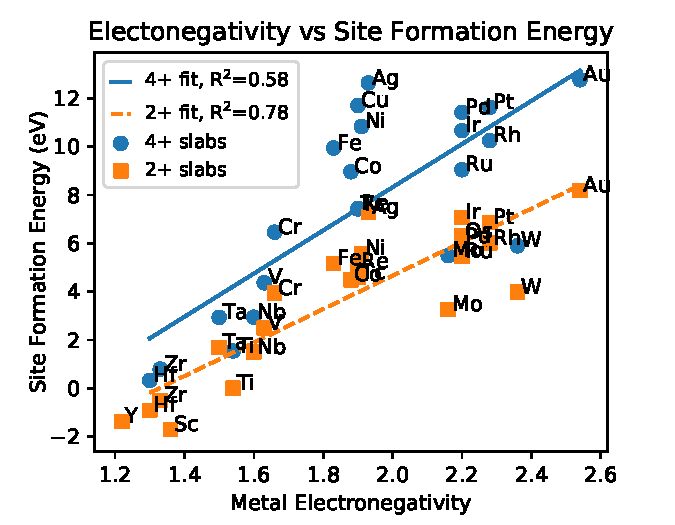
\includegraphics[width=0.8\linewidth]{Images/electronegativity_vs_formation.pdf}
\caption{Electronegativity vs formation energy of 2+ dopant site}
\end{figure}

\begin{figure}
\centering
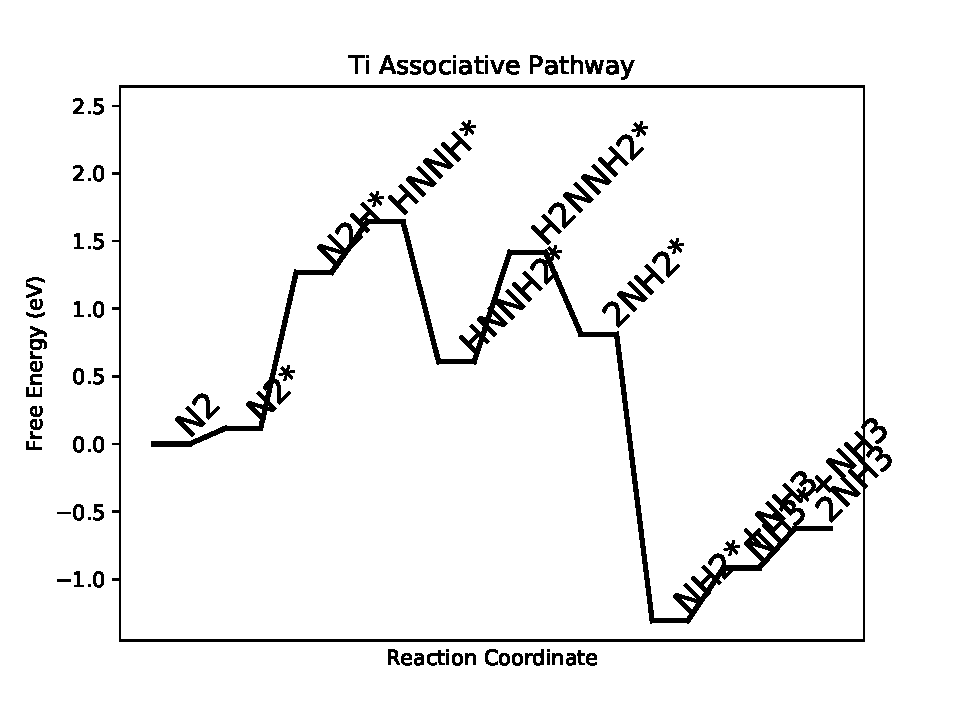
\includegraphics[width=0.8\linewidth]{data/plots/Ti_associative.pdf}
\end{figure}

\begin{figure}
\centering
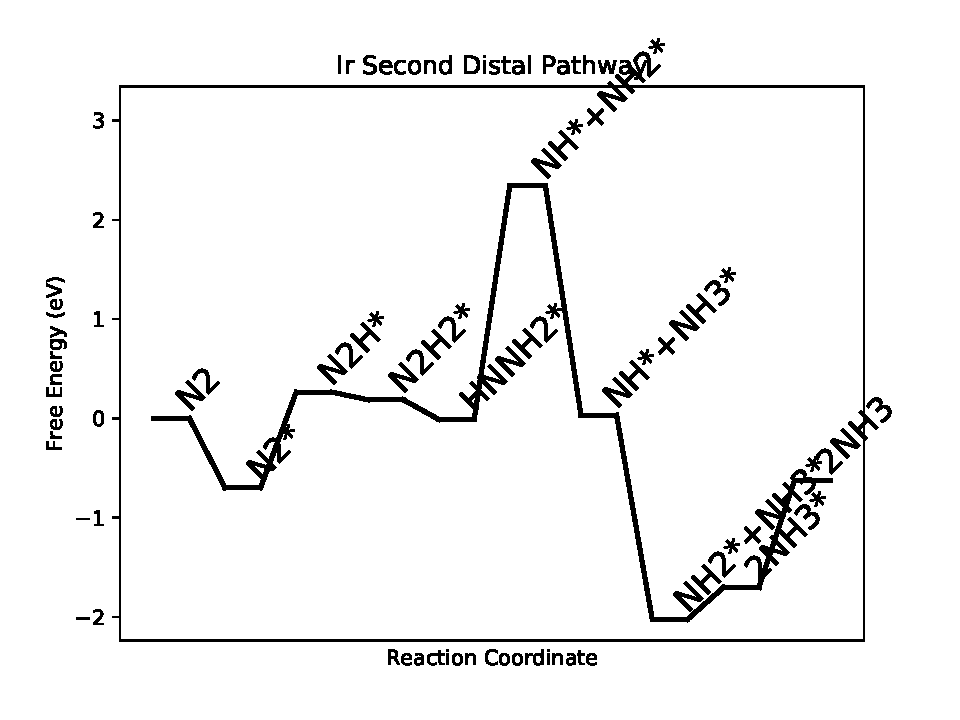
\includegraphics[width=0.8\linewidth]{data/plots/Ir_distal_2.pdf}
\end{figure}

\begin{figure}
\centering
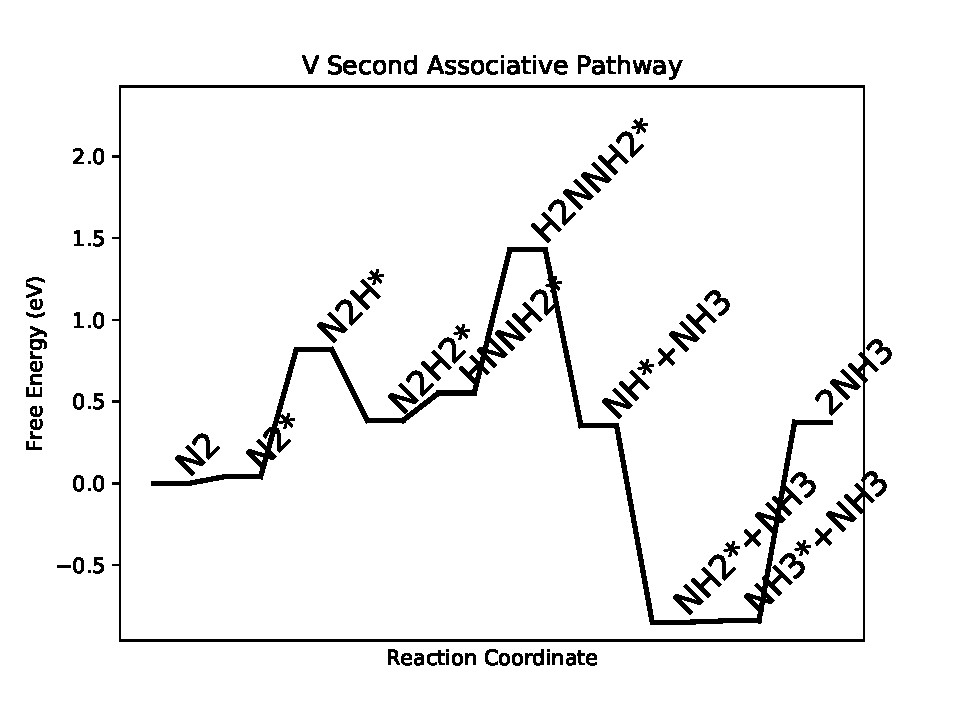
\includegraphics[width=0.8\linewidth]{data/plots/V_associative_2.pdf}
\end{figure}

\begin{figure}
\centering
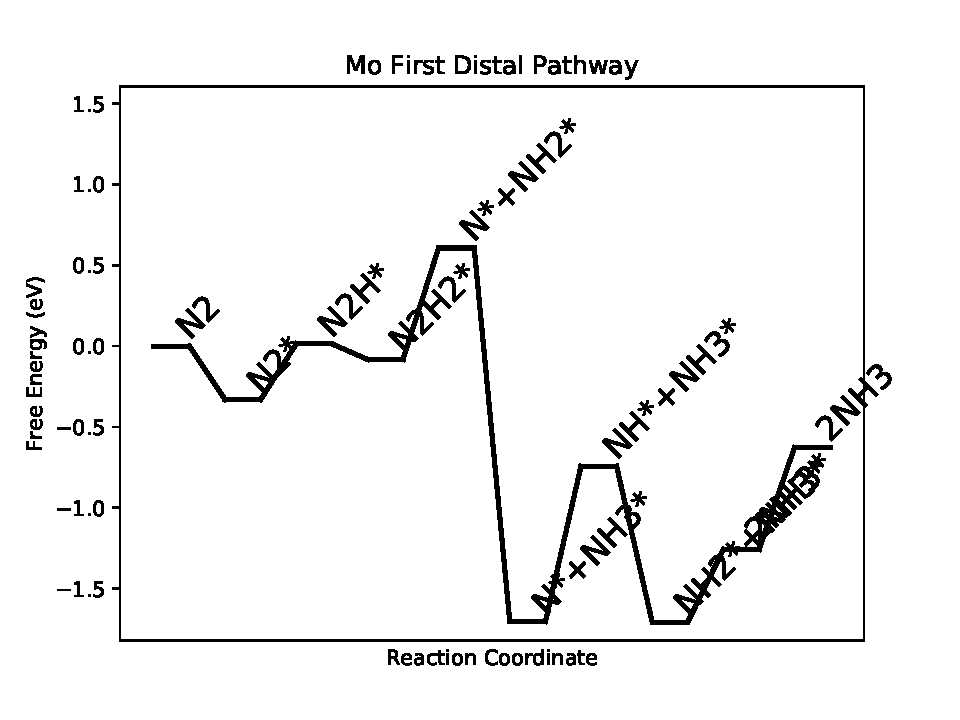
\includegraphics[width=0.8\linewidth]{data/plots/Mo_distal_1.pdf}
\end{figure}

\begin{figure}
\centering
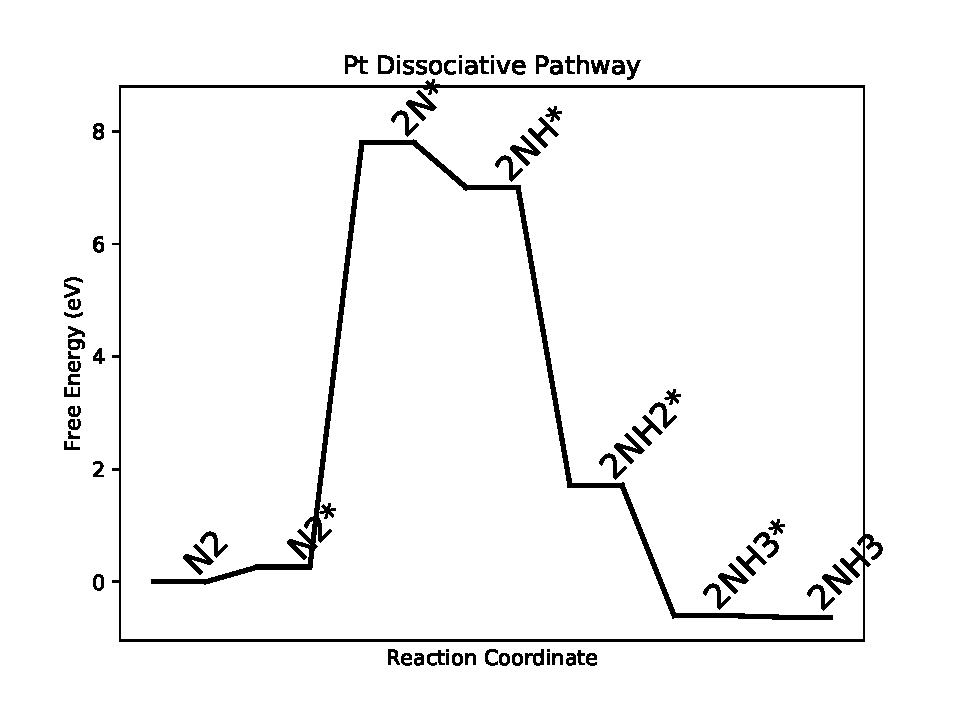
\includegraphics[width=0.8\linewidth]{data/plots/Pt_dissociative.pdf}
\end{figure}

\begin{figure}
\centering
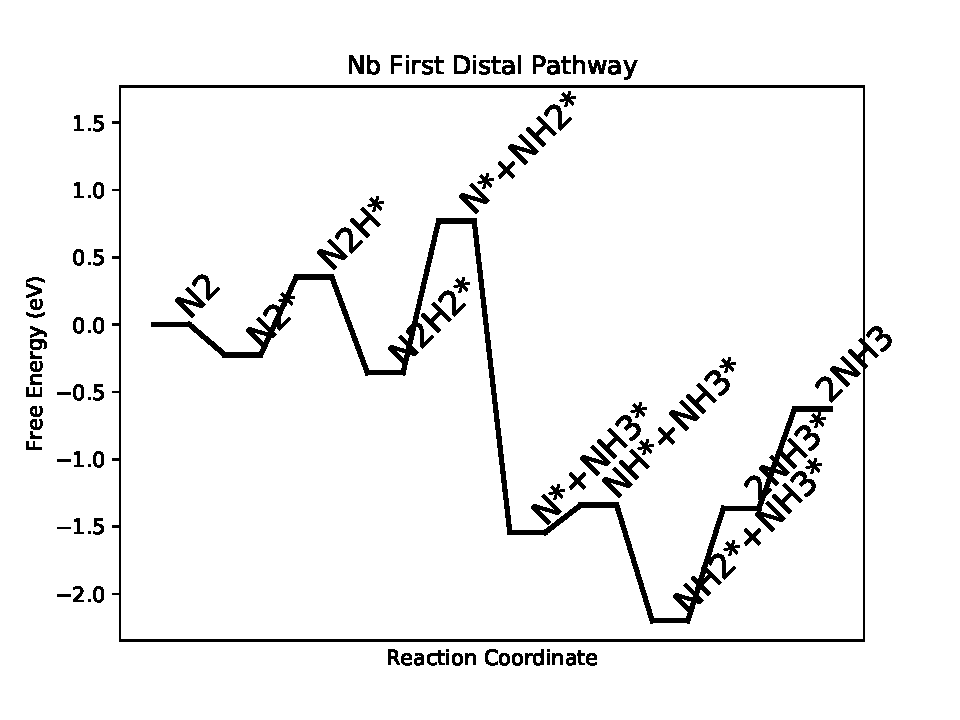
\includegraphics[width=0.8\linewidth]{data/plots/Nb_distal_1.pdf}
\end{figure}

\begin{figure}
\centering
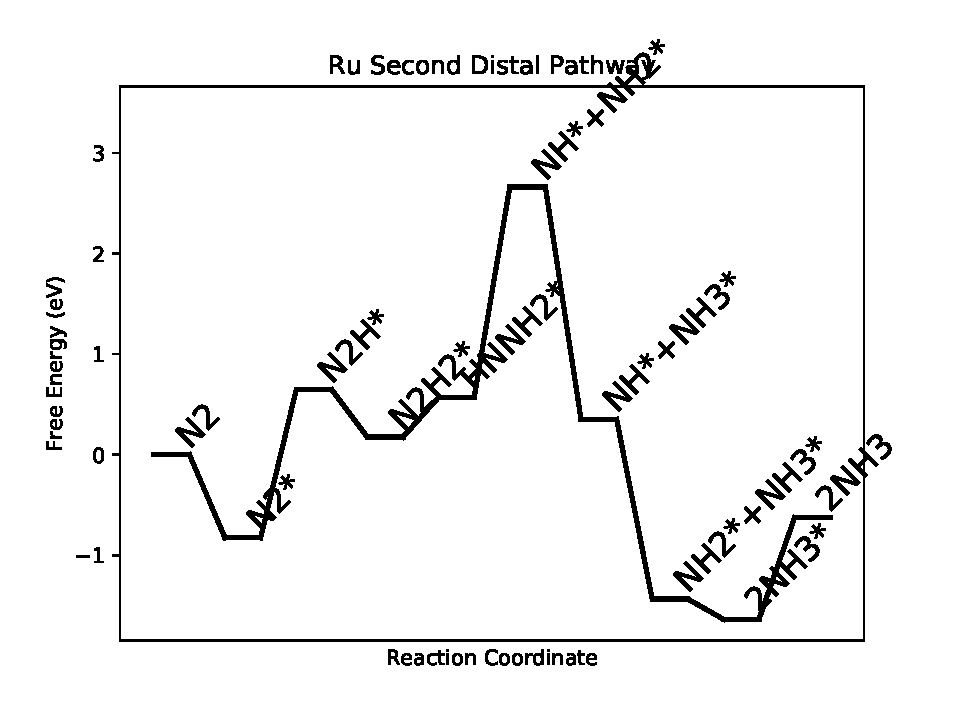
\includegraphics[width=0.8\linewidth]{data/plots/Ru_distal_2.pdf}
\end{figure}

\begin{figure}
\centering
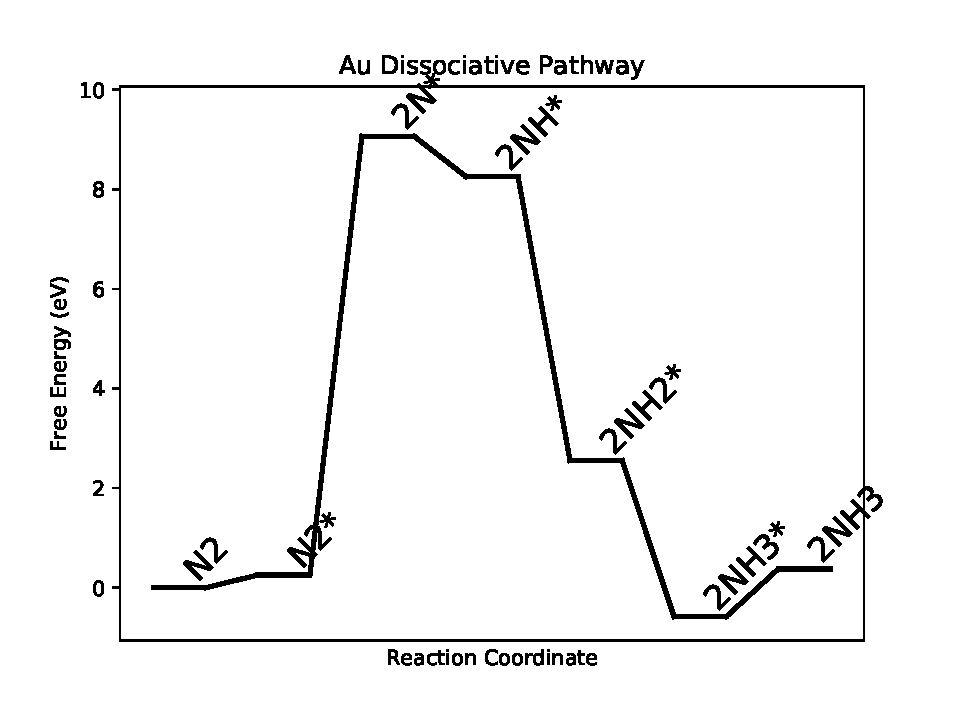
\includegraphics[width=0.8\linewidth]{data/plots/Au_dissociative.pdf}
\end{figure}

\begin{figure}
\centering
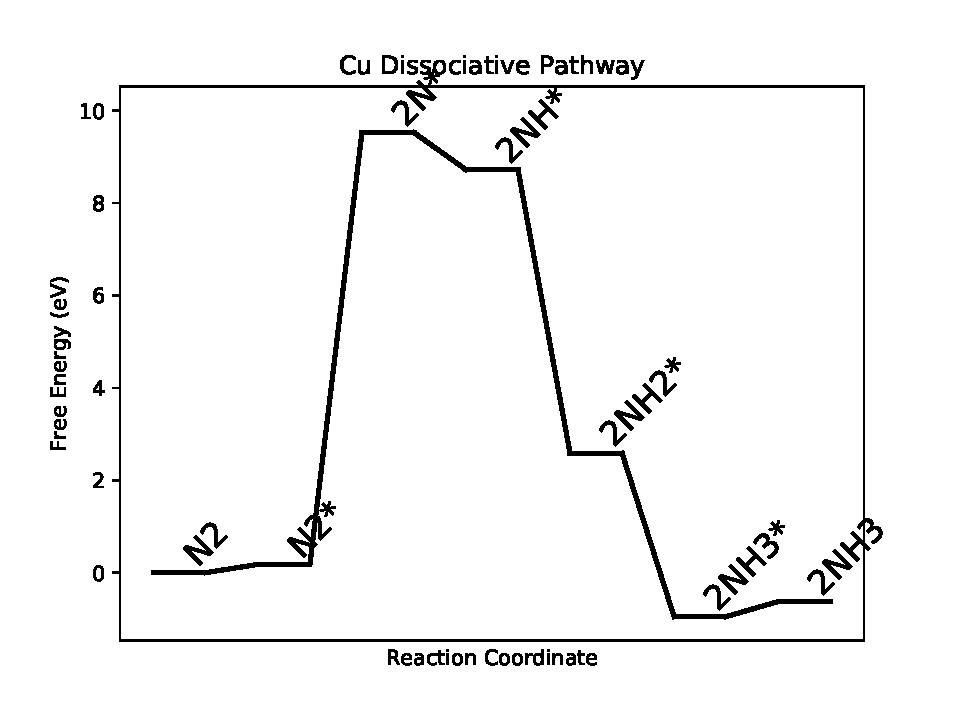
\includegraphics[width=0.8\linewidth]{data/plots/Cu_dissociative.pdf}
\end{figure}

\begin{figure}
\centering
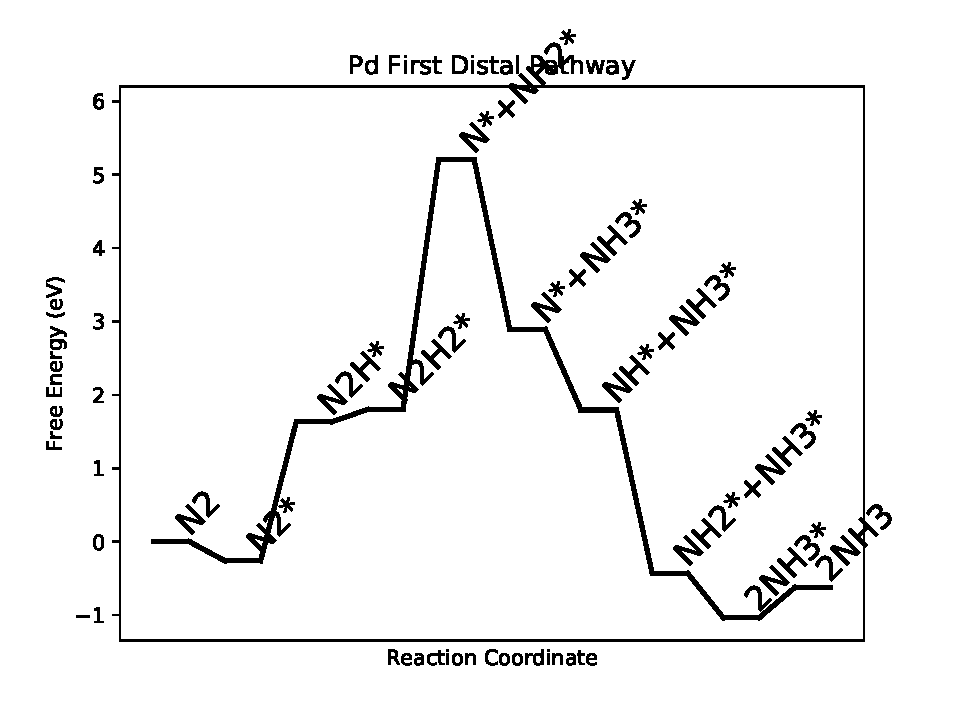
\includegraphics[width=0.8\linewidth]{data/plots/Pd_distal_1.pdf}
\end{figure}

\begin{figure}
\centering
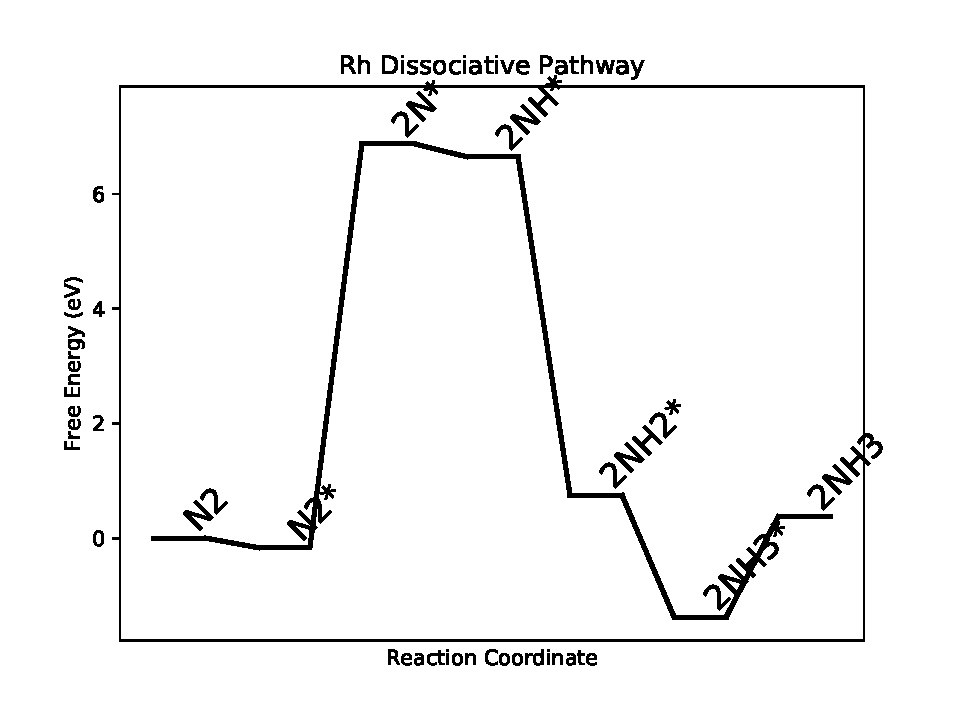
\includegraphics[width=0.8\linewidth]{data/plots/Rh_dissociative.pdf}
\end{figure}

\begin{figure}
\centering
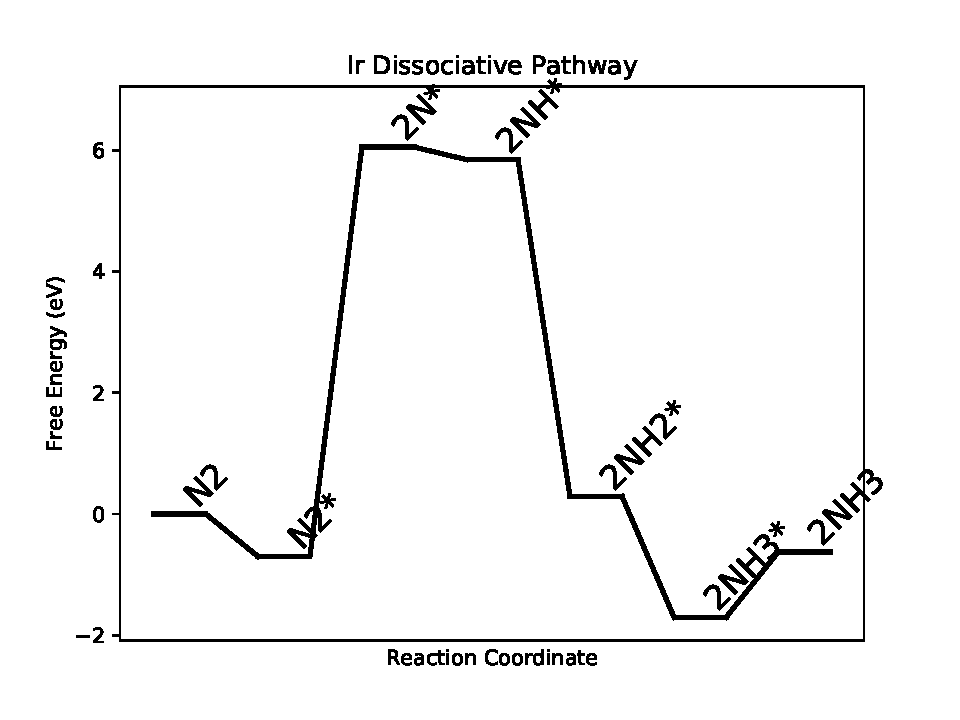
\includegraphics[width=0.8\linewidth]{data/plots/Ir_dissociative.pdf}
\end{figure}

\begin{figure}
\centering
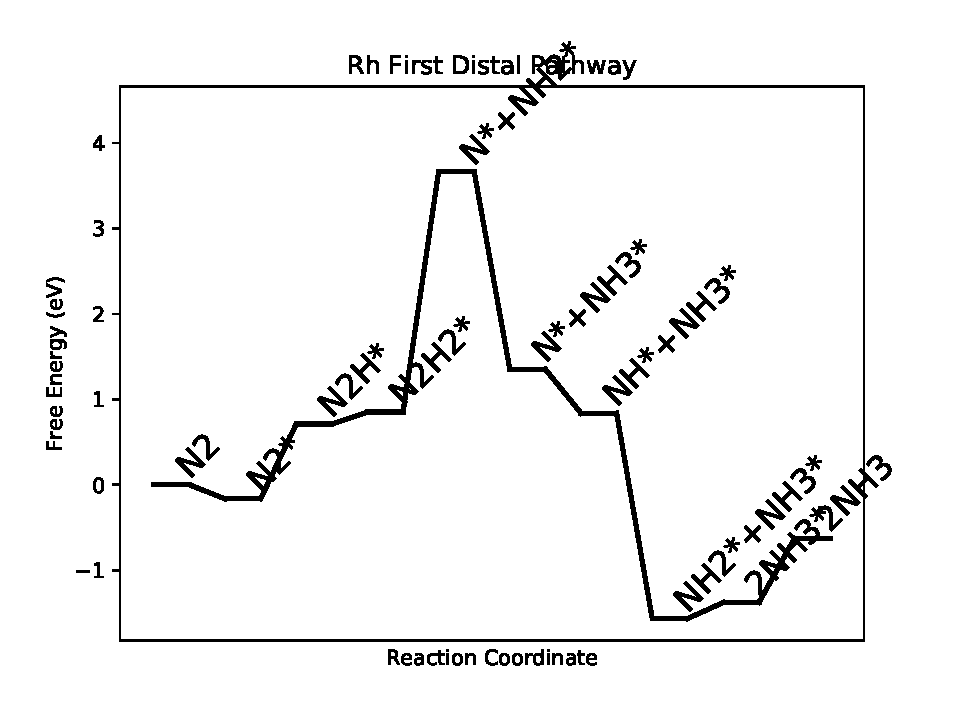
\includegraphics[width=0.8\linewidth]{data/plots/Rh_distal_1.pdf}
\end{figure}

\begin{figure}
\centering
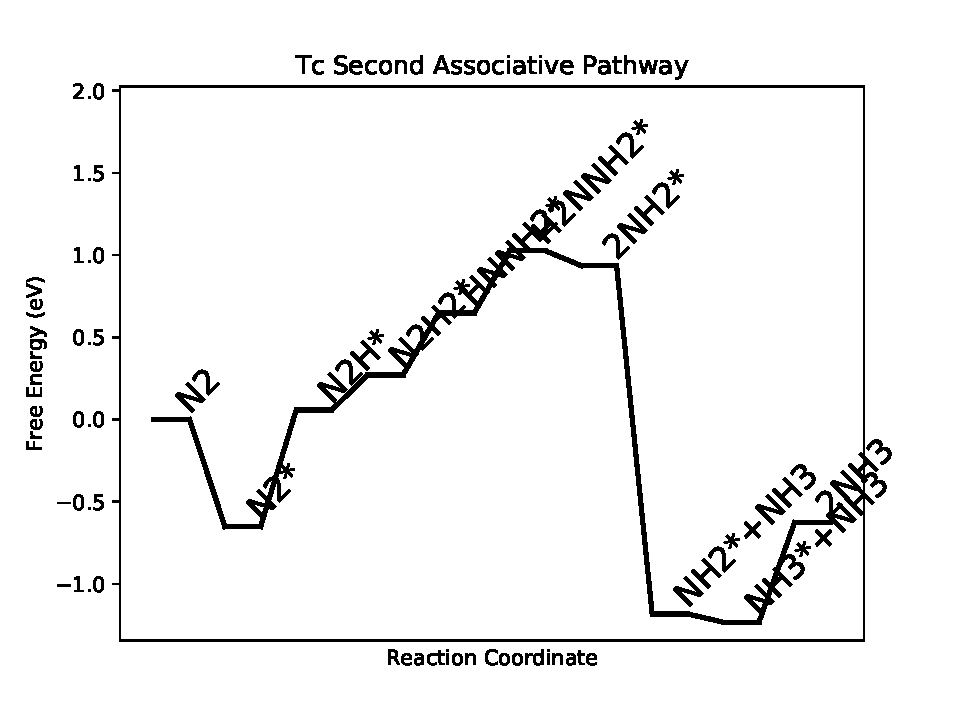
\includegraphics[width=0.8\linewidth]{data/plots/Tc_associative_2.pdf}
\end{figure}

\begin{figure}
\centering
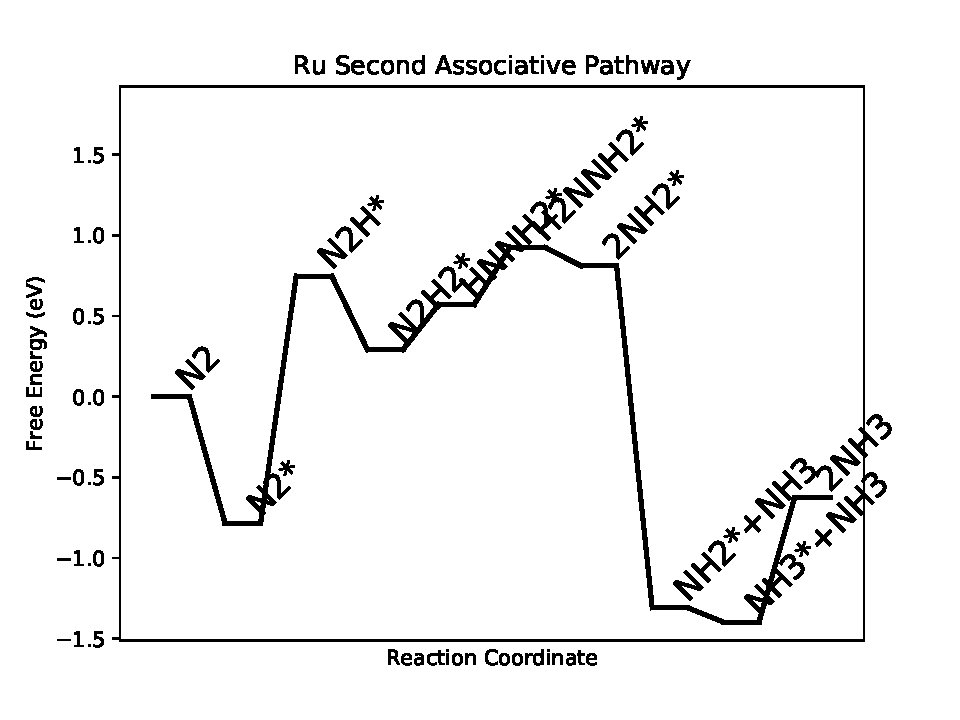
\includegraphics[width=0.8\linewidth]{data/plots/Ru_associative_2.pdf}
\end{figure}

\begin{figure}
\centering
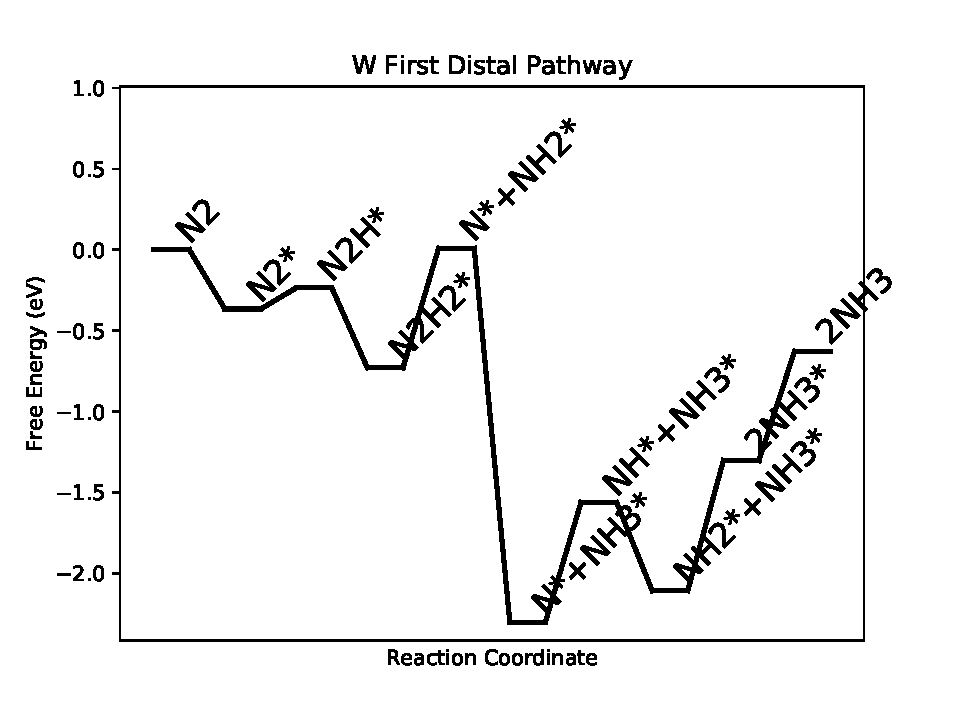
\includegraphics[width=0.8\linewidth]{data/plots/W_distal_1.pdf}
\end{figure}

\begin{figure}
\centering
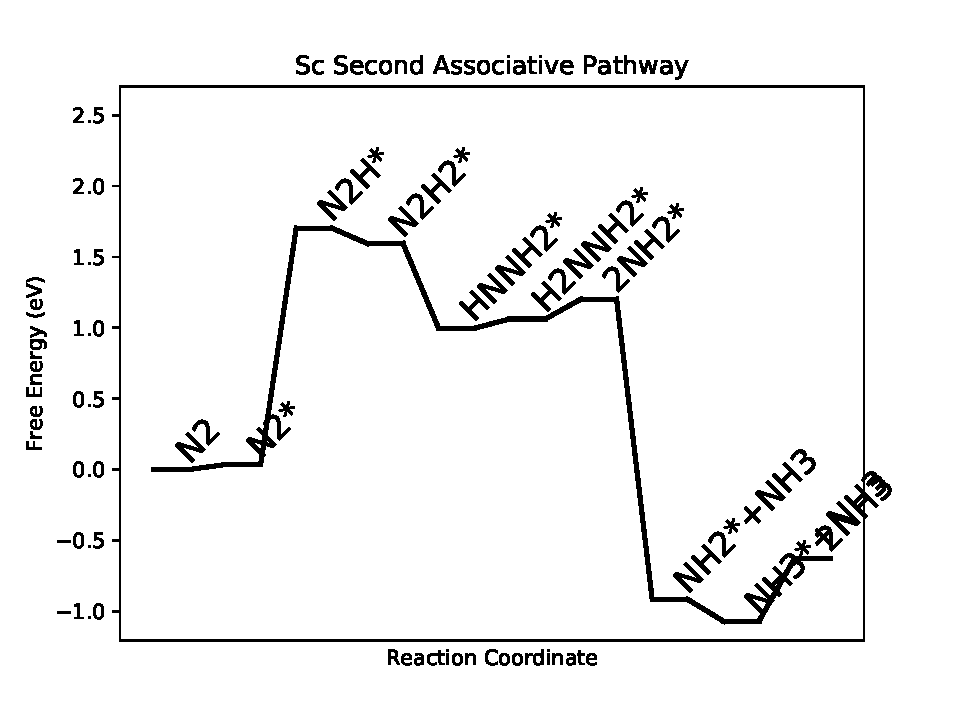
\includegraphics[width=0.8\linewidth]{data/plots/Sc_associative_2.pdf}
\end{figure}

\begin{figure}
\centering
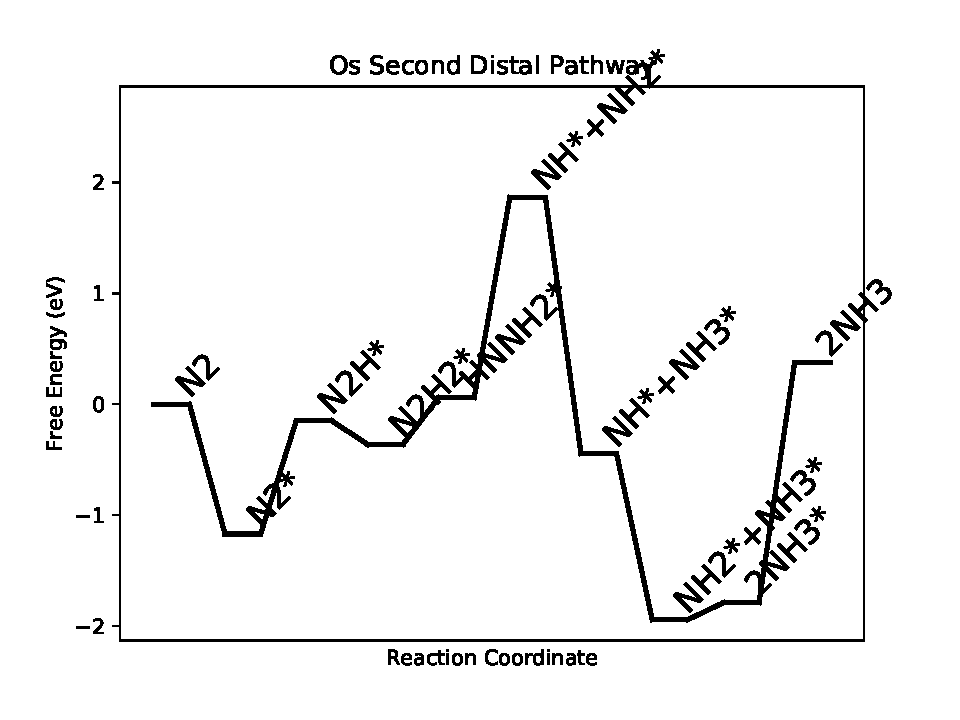
\includegraphics[width=0.8\linewidth]{data/plots/Os_distal_2.pdf}
\end{figure}

\begin{figure}
\centering
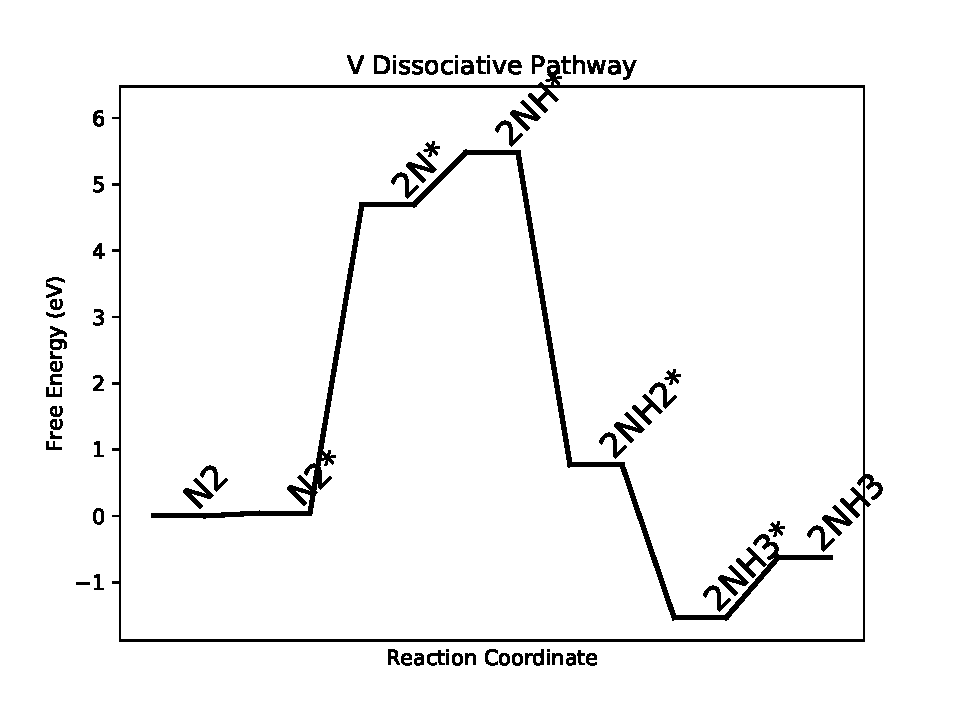
\includegraphics[width=0.8\linewidth]{data/plots/V_dissociative.pdf}
\end{figure}

\begin{figure}
\centering
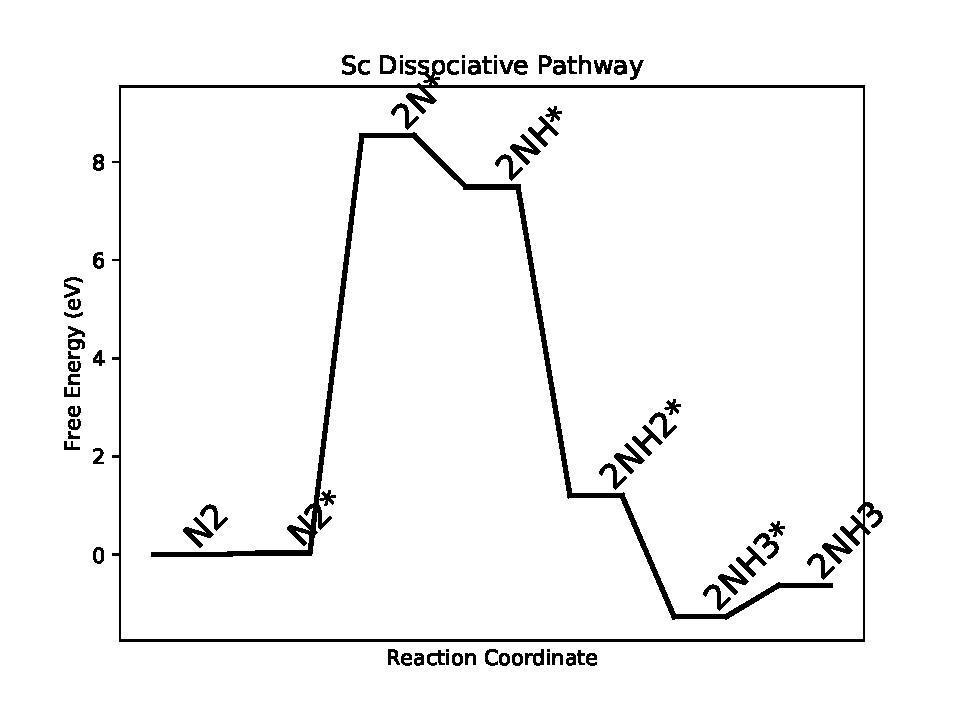
\includegraphics[width=0.8\linewidth]{data/plots/Sc_dissociative.pdf}
\end{figure}

\begin{figure}
\centering
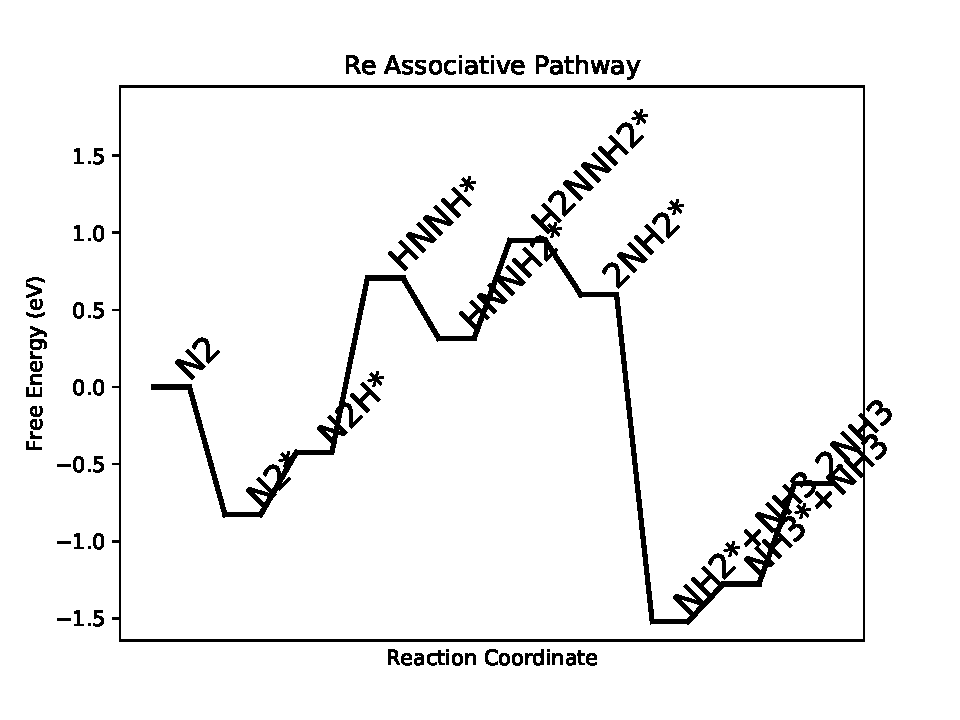
\includegraphics[width=0.8\linewidth]{data/plots/Re_associative.pdf}
\end{figure}

\begin{figure}
\centering
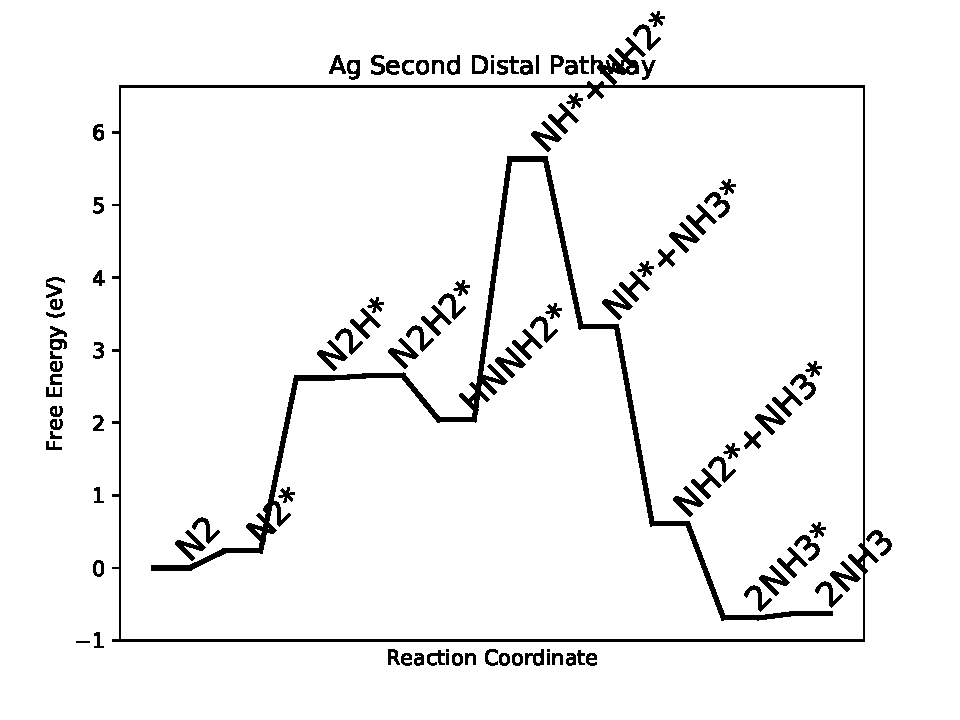
\includegraphics[width=0.8\linewidth]{data/plots/Ag_distal_2.pdf}
\end{figure}

\begin{figure}
\centering
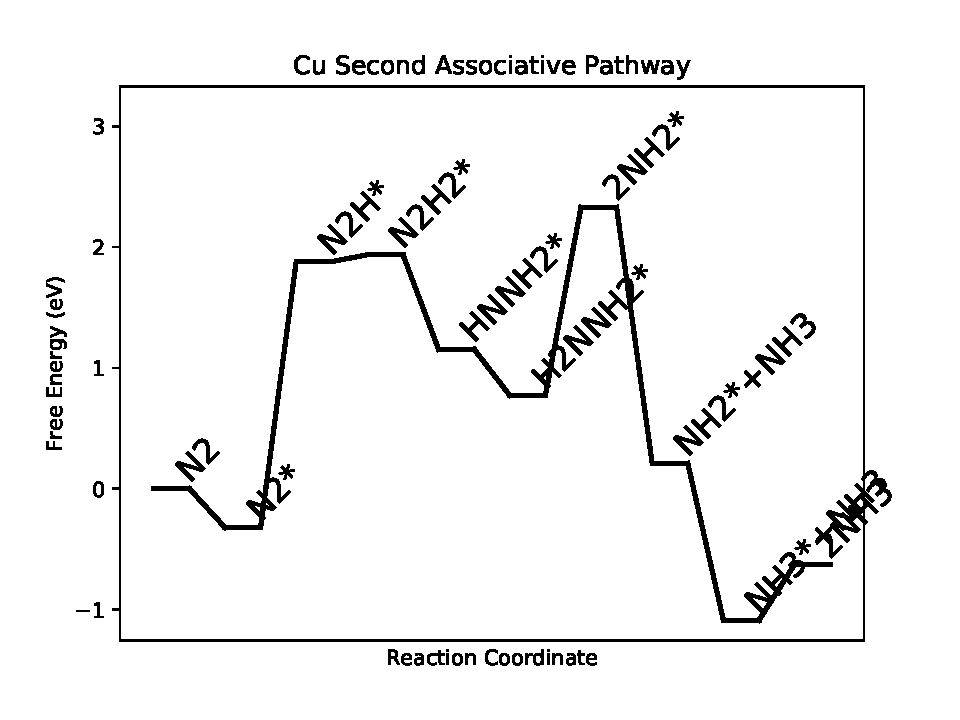
\includegraphics[width=0.8\linewidth]{data/plots/Cu_associative_2.pdf}
\end{figure}

\begin{figure}
\centering
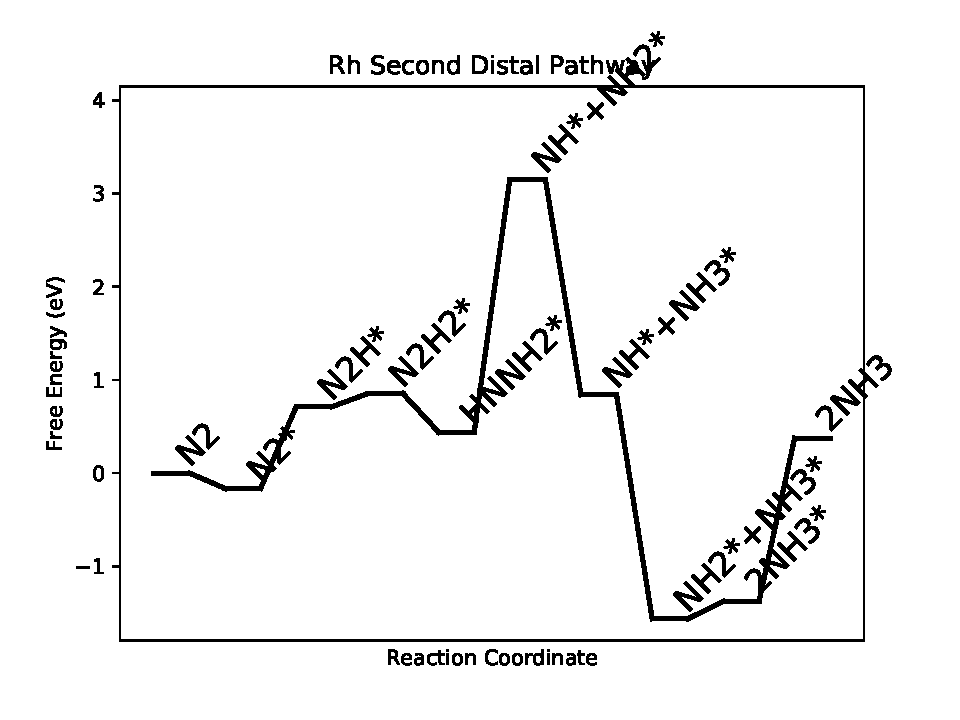
\includegraphics[width=0.8\linewidth]{data/plots/Rh_distal_2.pdf}
\end{figure}

\begin{figure}
\centering
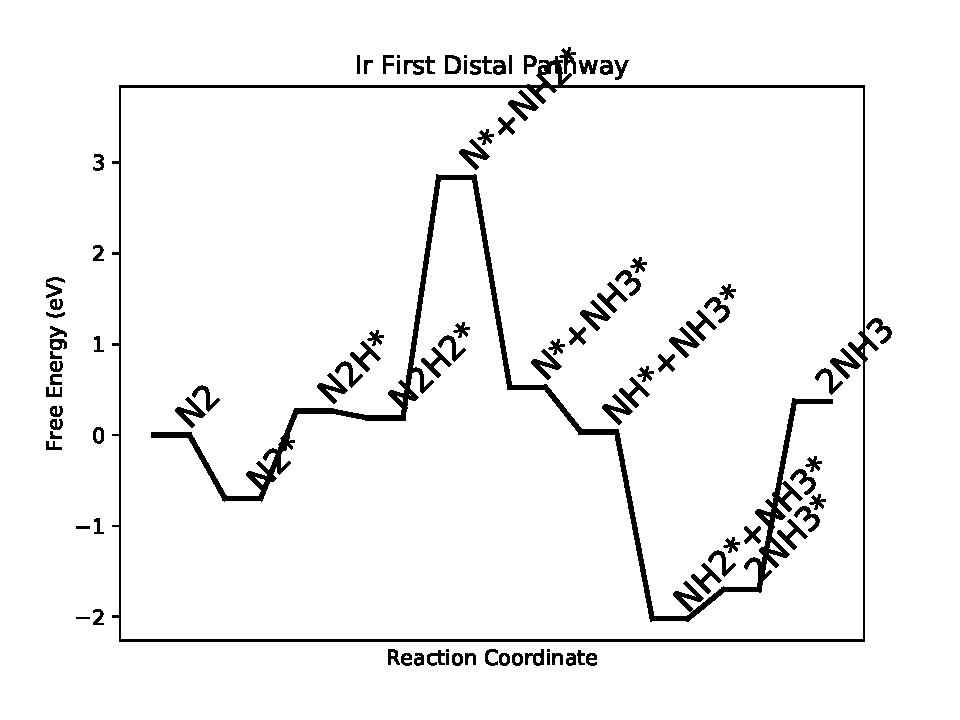
\includegraphics[width=0.8\linewidth]{data/plots/Ir_distal_1.pdf}
\end{figure}

\begin{figure}
\centering
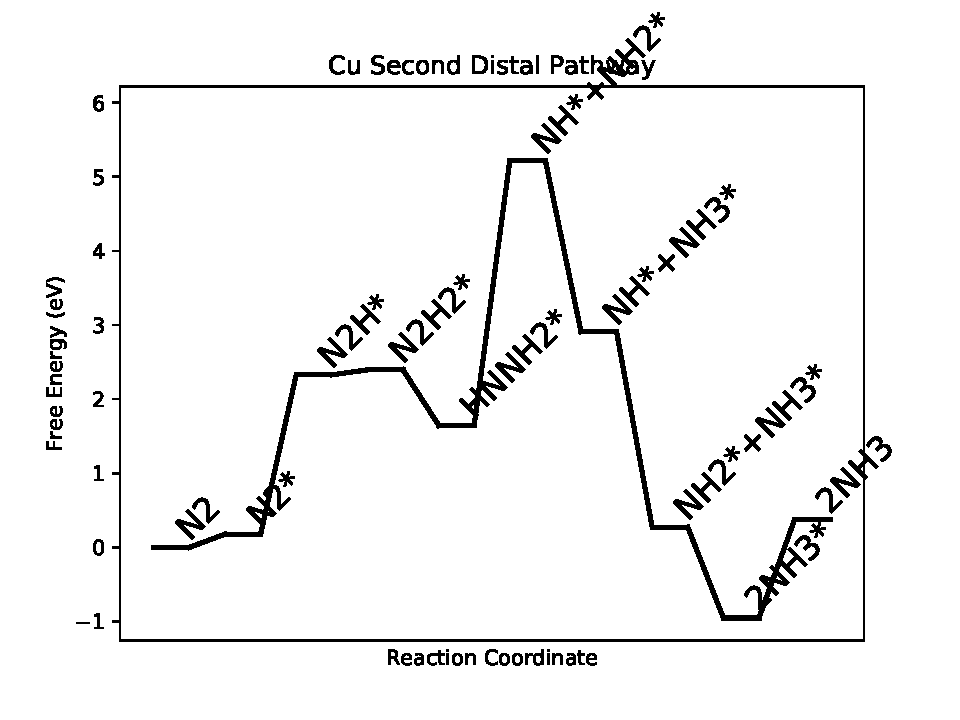
\includegraphics[width=0.8\linewidth]{data/plots/Cu_distal_2.pdf}
\end{figure}

\begin{figure}
\centering
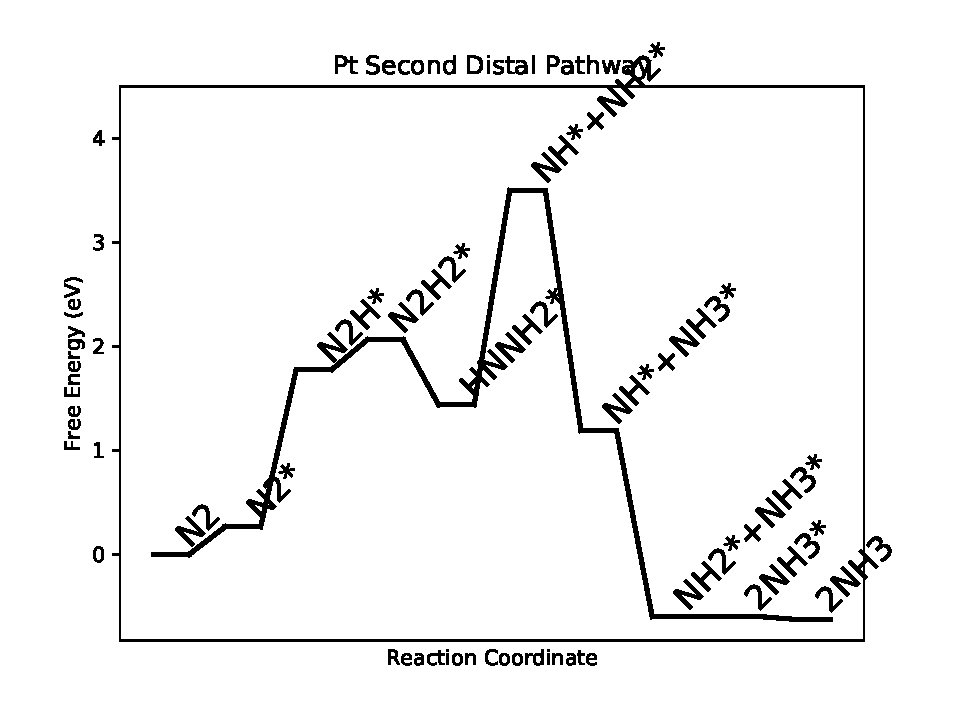
\includegraphics[width=0.8\linewidth]{data/plots/Pt_distal_2.pdf}
\end{figure}

\begin{figure}
\centering
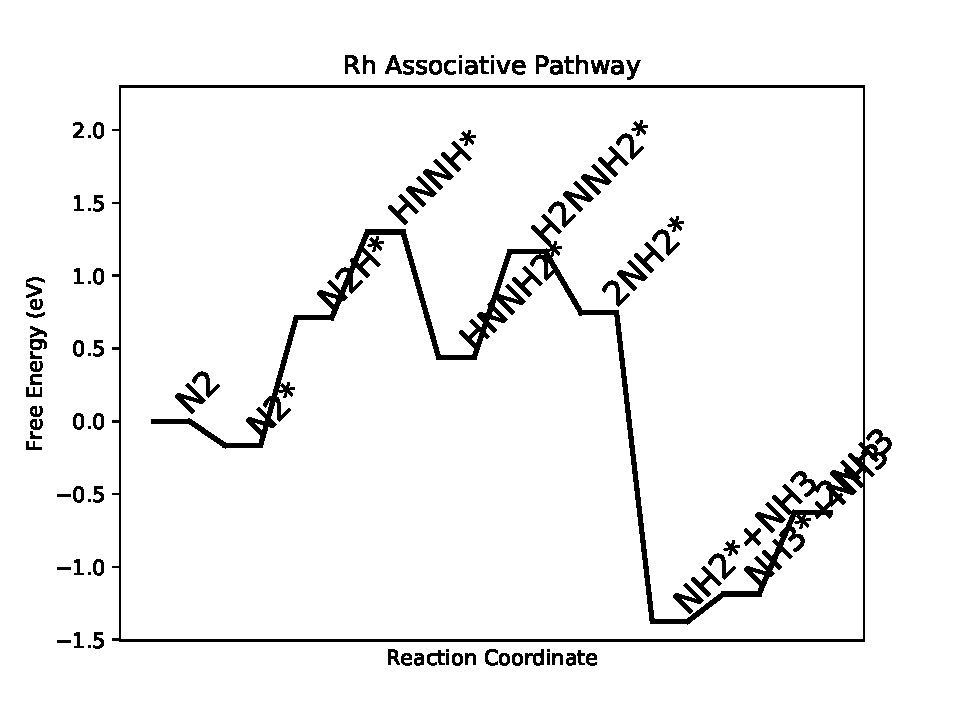
\includegraphics[width=0.8\linewidth]{data/plots/Rh_associative.pdf}
\end{figure}

\begin{figure}
\centering
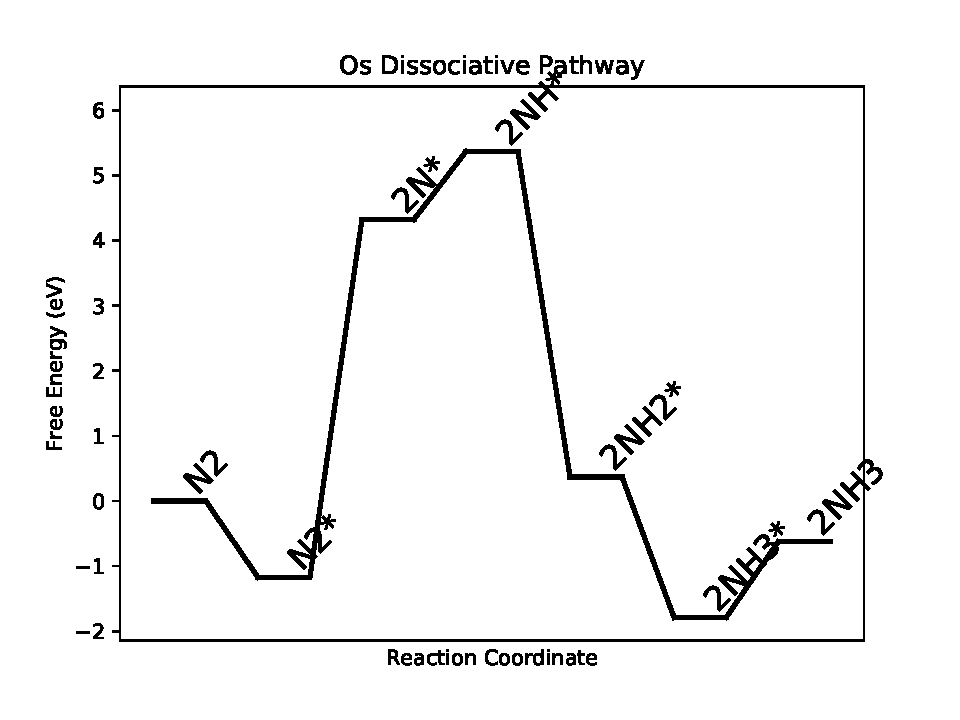
\includegraphics[width=0.8\linewidth]{data/plots/Os_dissociative.pdf}
\end{figure}

\begin{figure}
\centering
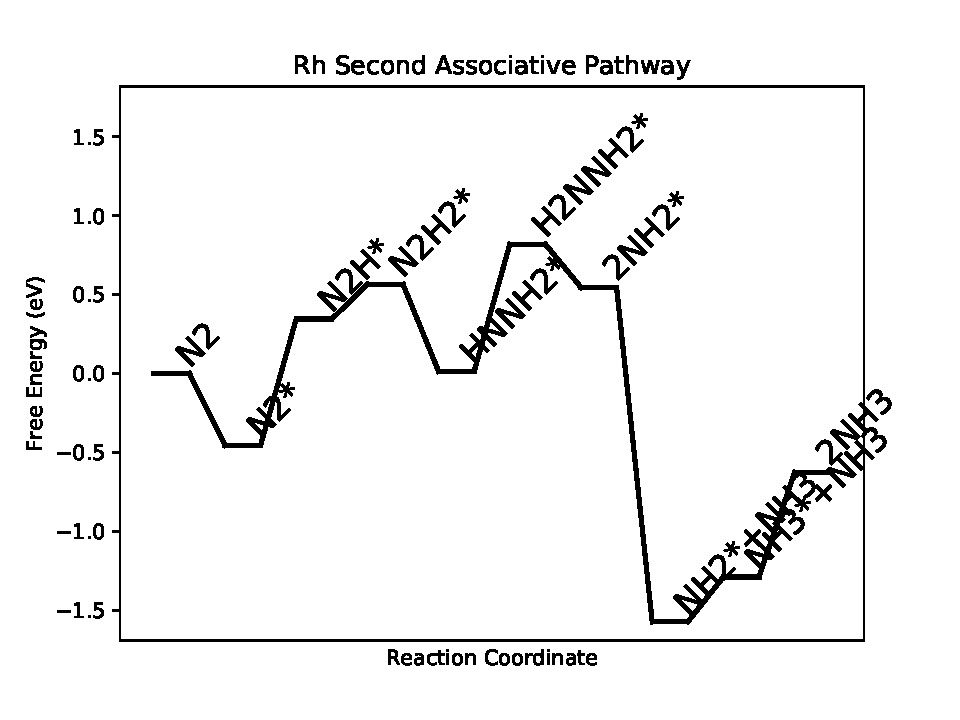
\includegraphics[width=0.8\linewidth]{data/plots/Rh_associative_2.pdf}
\end{figure}

\begin{figure}
\centering
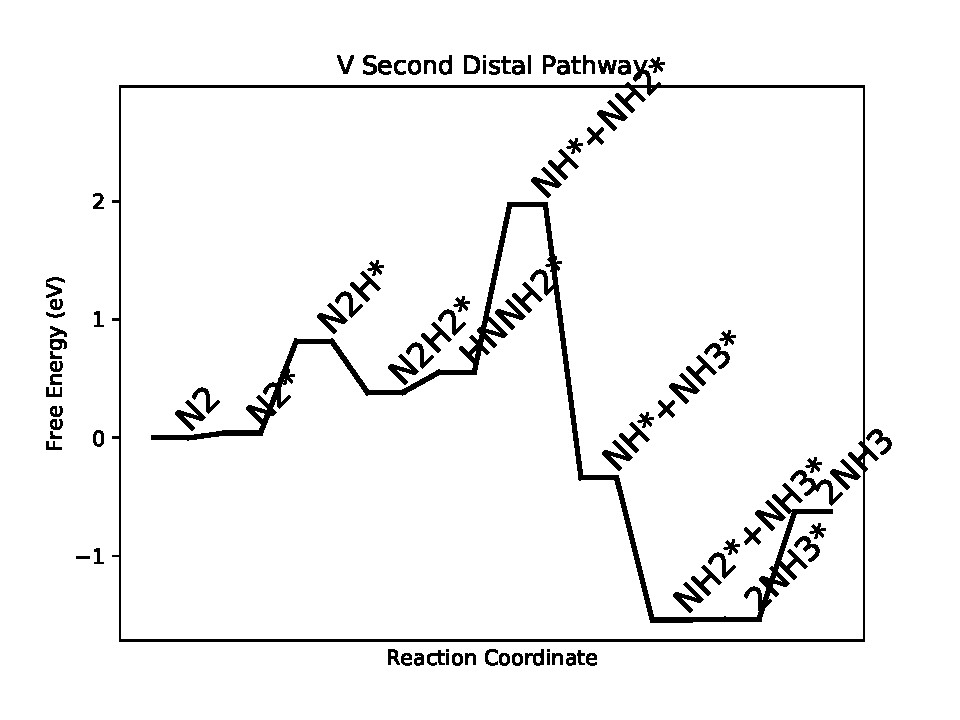
\includegraphics[width=0.8\linewidth]{data/plots/V_distal_2.pdf}
\end{figure}

\begin{figure}
\centering
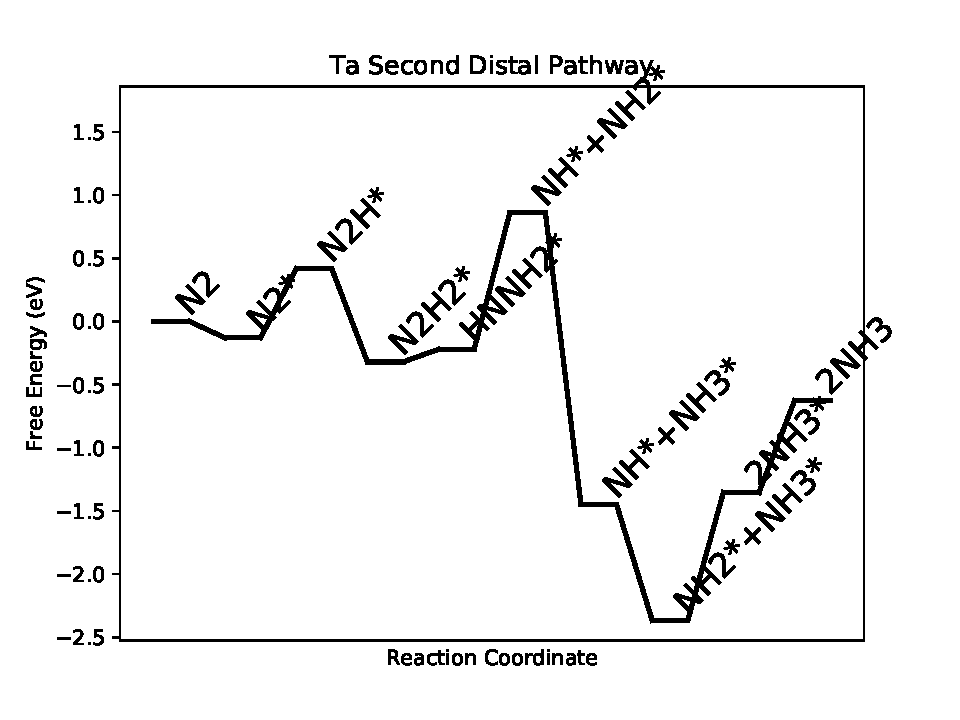
\includegraphics[width=0.8\linewidth]{data/plots/Ta_distal_2.pdf}
\end{figure}

\begin{figure}
\centering
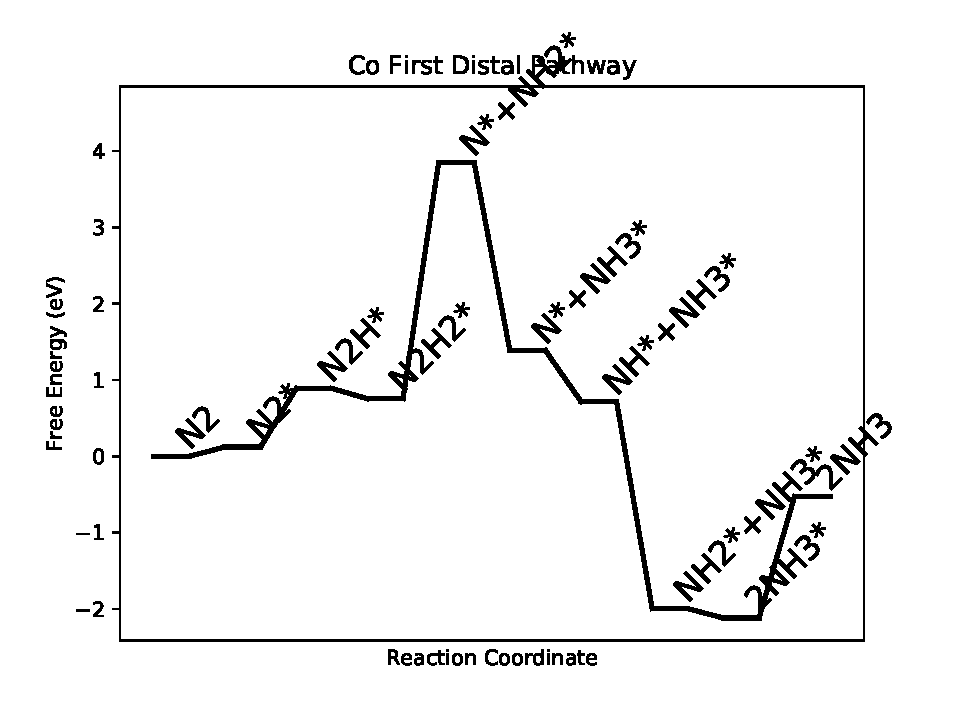
\includegraphics[width=0.8\linewidth]{data/plots/Co_distal_1.pdf}
\end{figure}

\begin{figure}
\centering
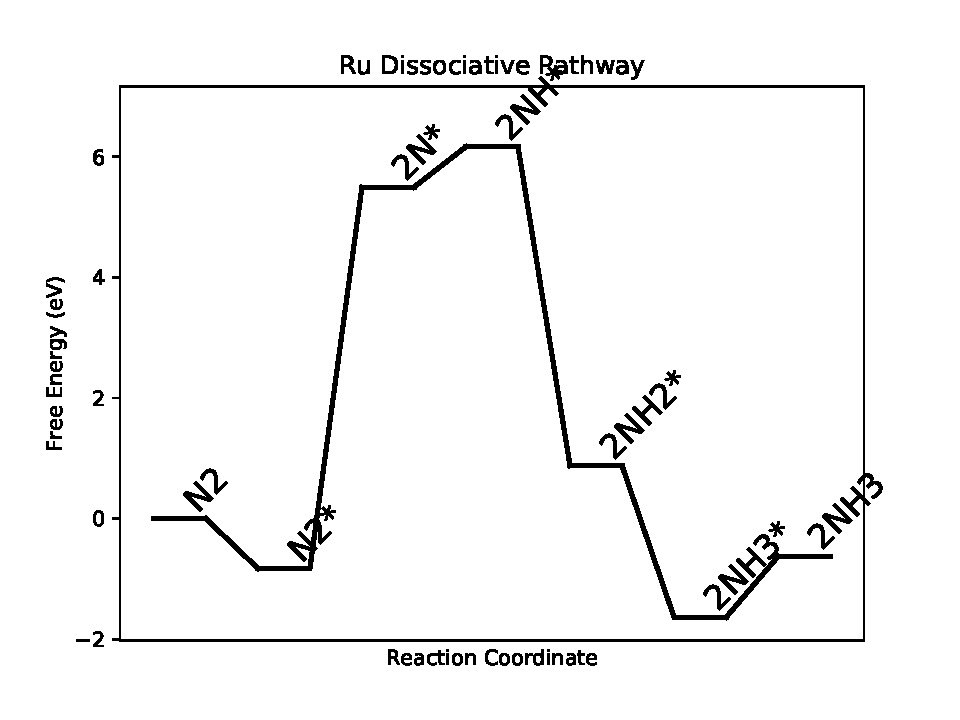
\includegraphics[width=0.8\linewidth]{data/plots/Ru_dissociative.pdf}
\end{figure}

\begin{figure}
\centering
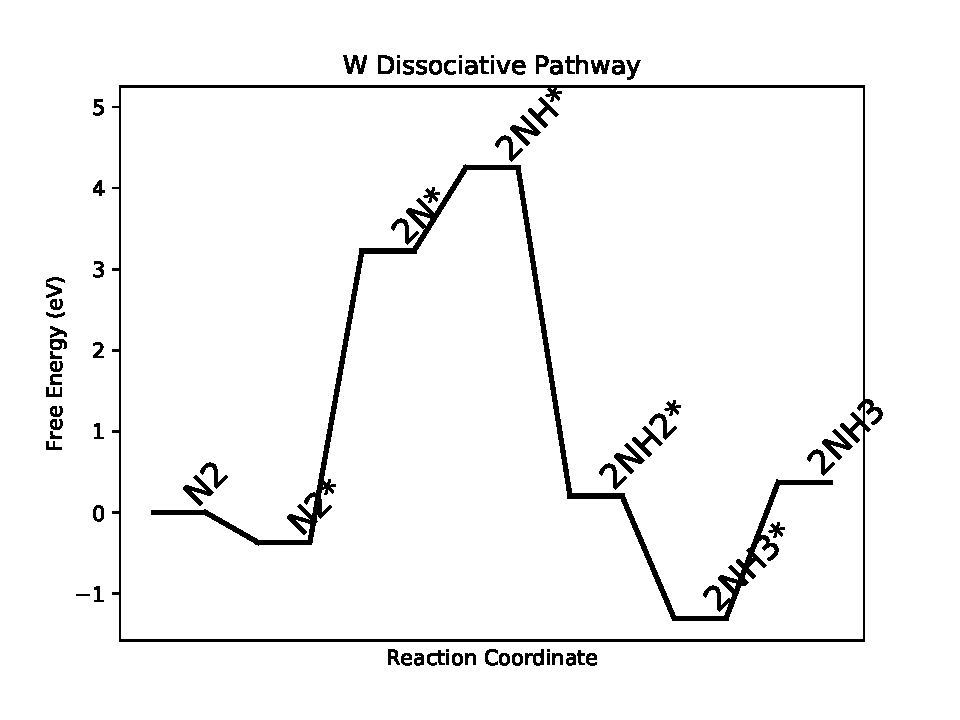
\includegraphics[width=0.8\linewidth]{data/plots/W_dissociative.pdf}
\end{figure}

\begin{figure}
\centering
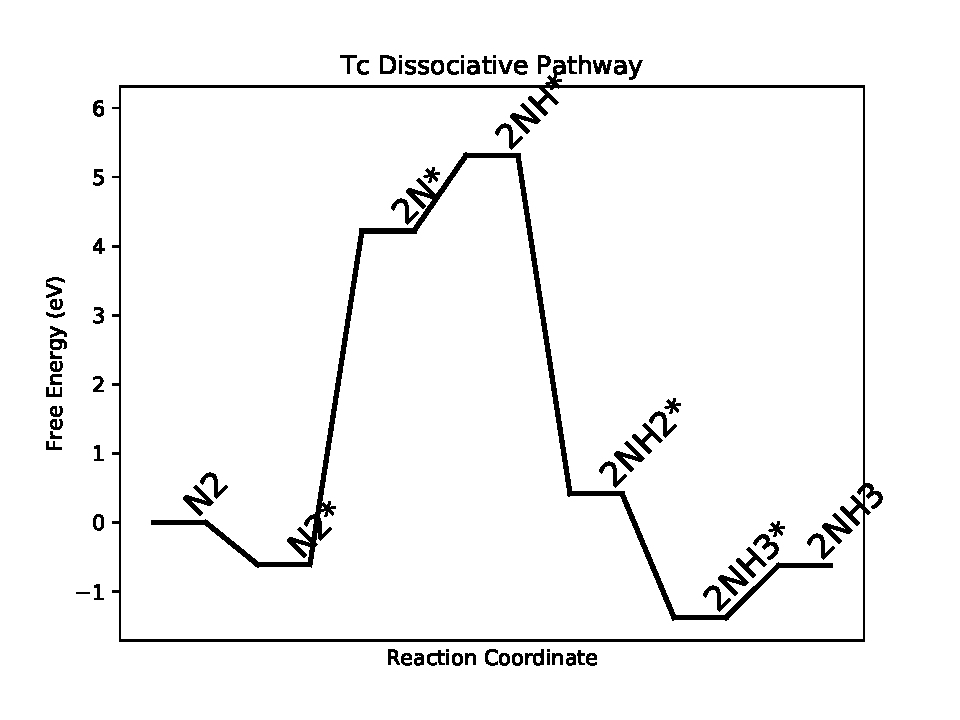
\includegraphics[width=0.8\linewidth]{data/plots/Tc_dissociative.pdf}
\end{figure}

\begin{figure}
\centering
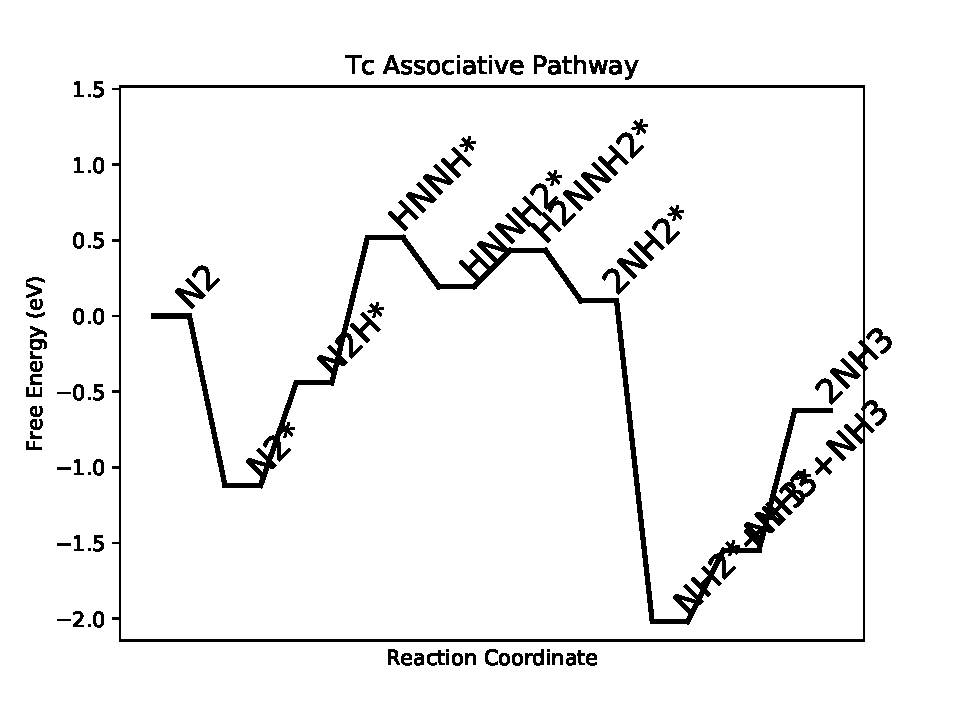
\includegraphics[width=0.8\linewidth]{data/plots/Tc_associative.pdf}
\end{figure}

\begin{figure}
\centering
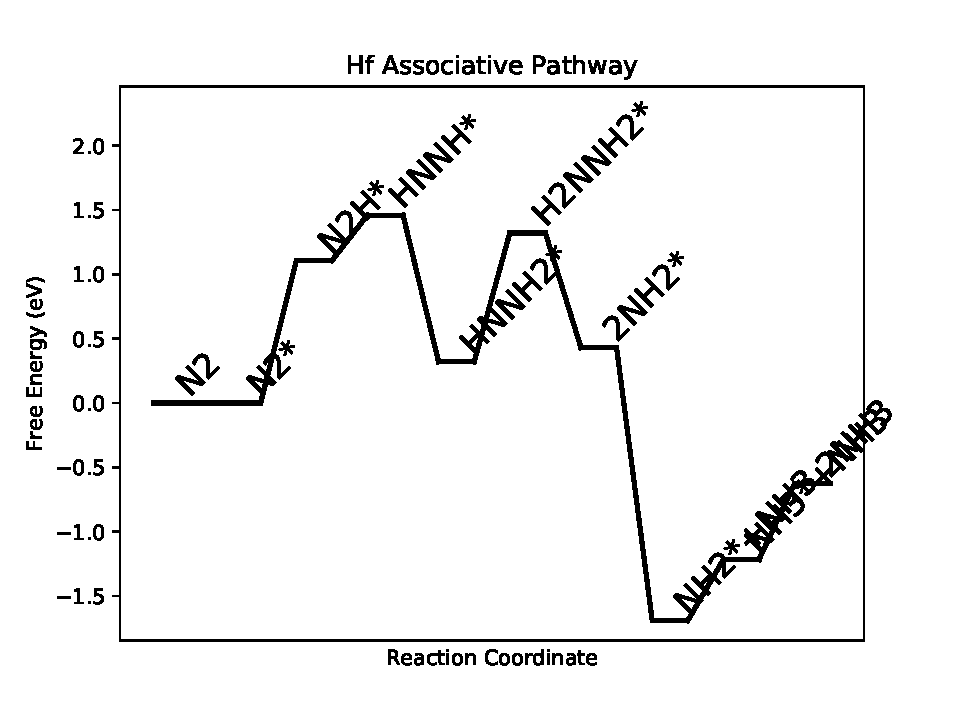
\includegraphics[width=0.8\linewidth]{data/plots/Hf_associative.pdf}
\end{figure}

\begin{figure}
\centering
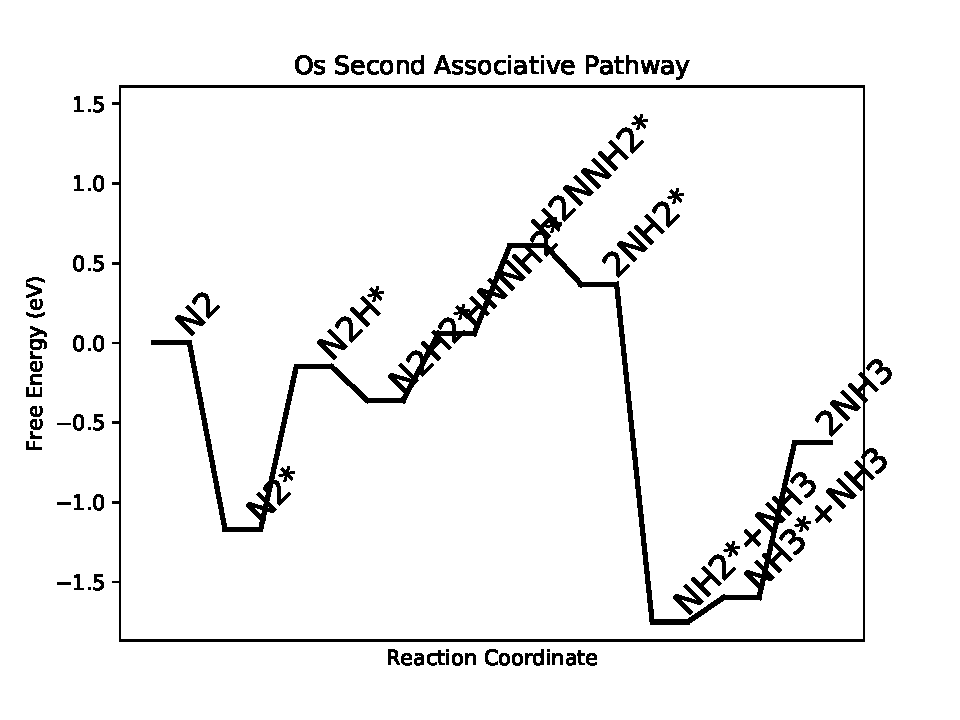
\includegraphics[width=0.8\linewidth]{data/plots/Os_associative_2.pdf}
\end{figure}

\begin{figure}
\centering
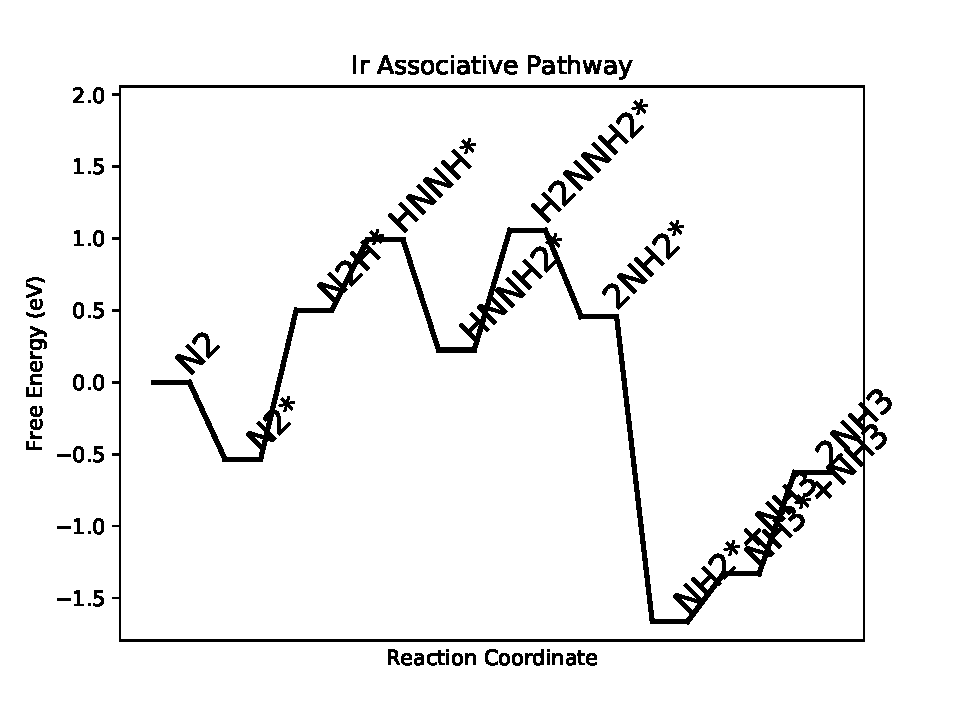
\includegraphics[width=0.8\linewidth]{data/plots/Ir_associative.pdf}
\end{figure}

\begin{figure}
\centering
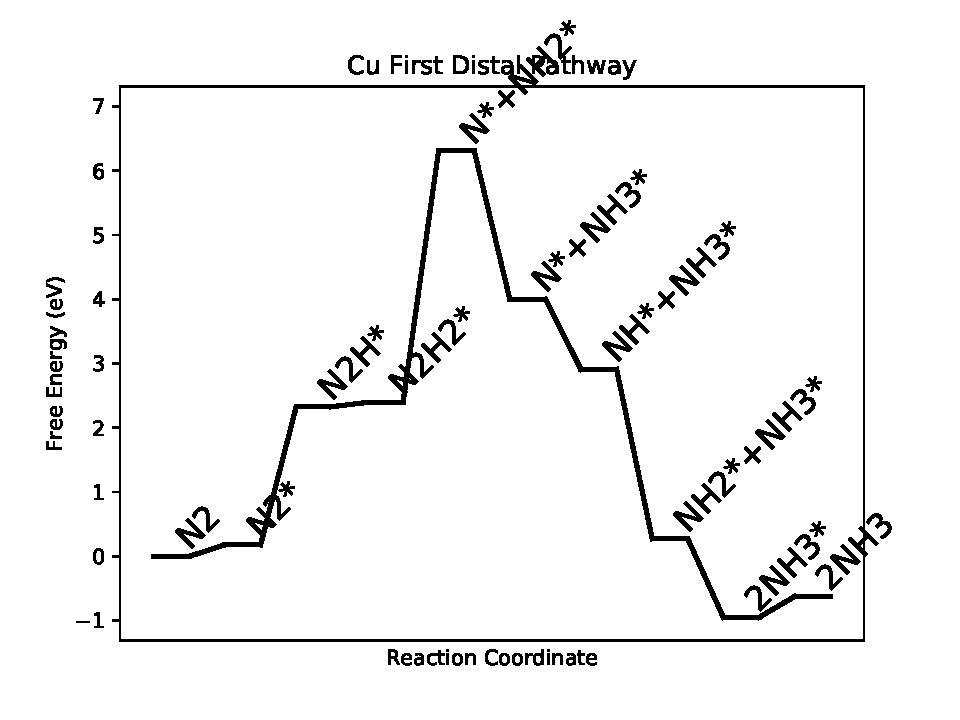
\includegraphics[width=0.8\linewidth]{data/plots/Cu_distal_1.pdf}
\end{figure}

\begin{figure}
\centering
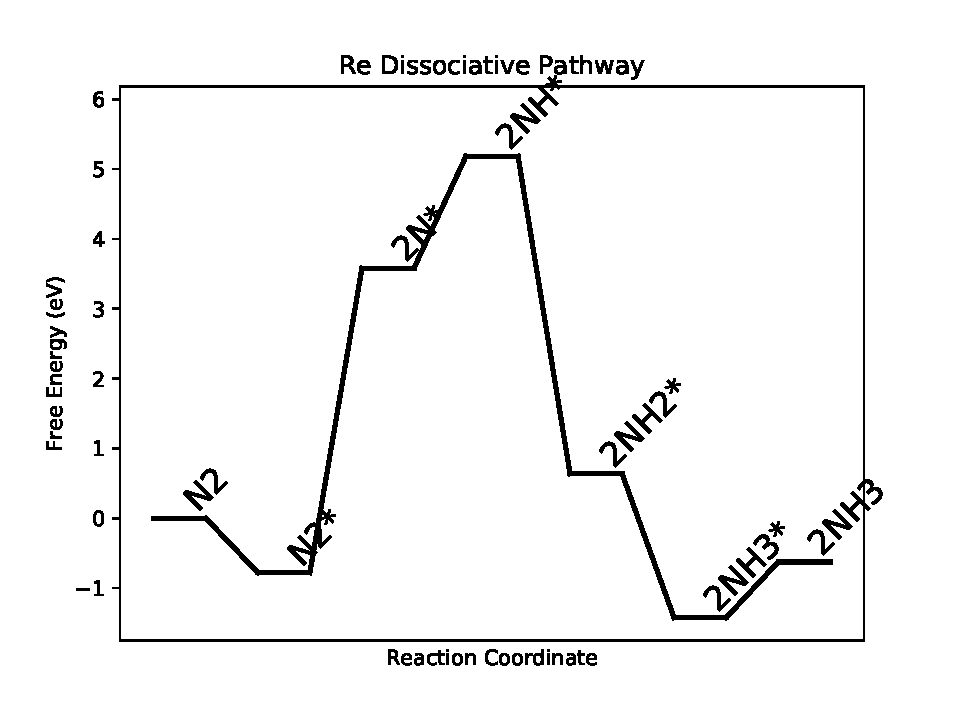
\includegraphics[width=0.8\linewidth]{data/plots/Re_dissociative.pdf}
\end{figure}

\begin{figure}
\centering
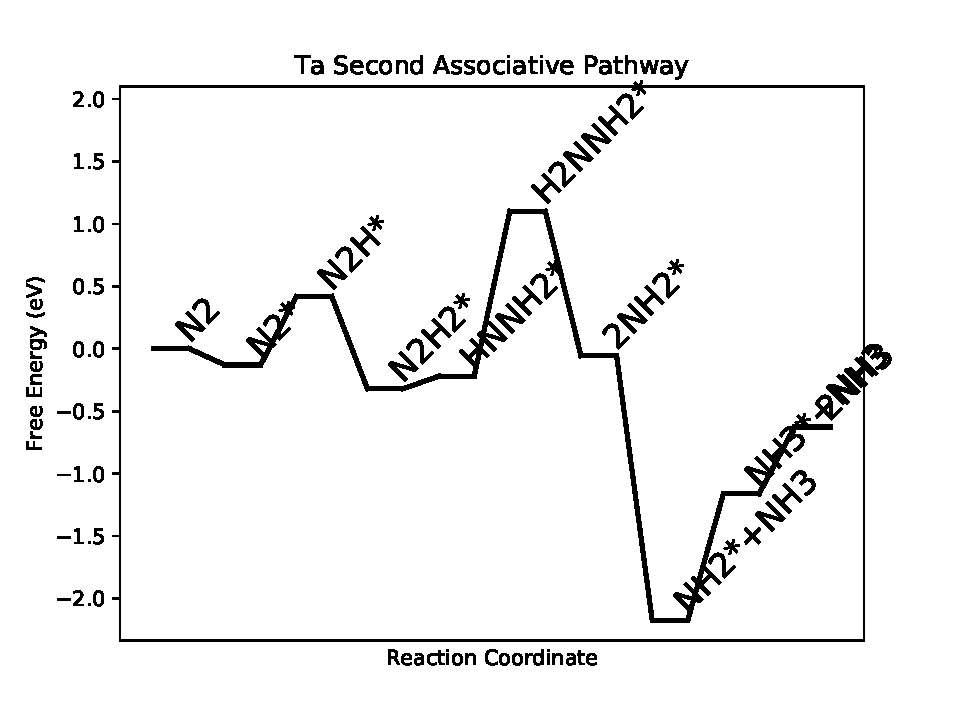
\includegraphics[width=0.8\linewidth]{data/plots/Ta_associative_2.pdf}
\end{figure}

\begin{figure}
\centering
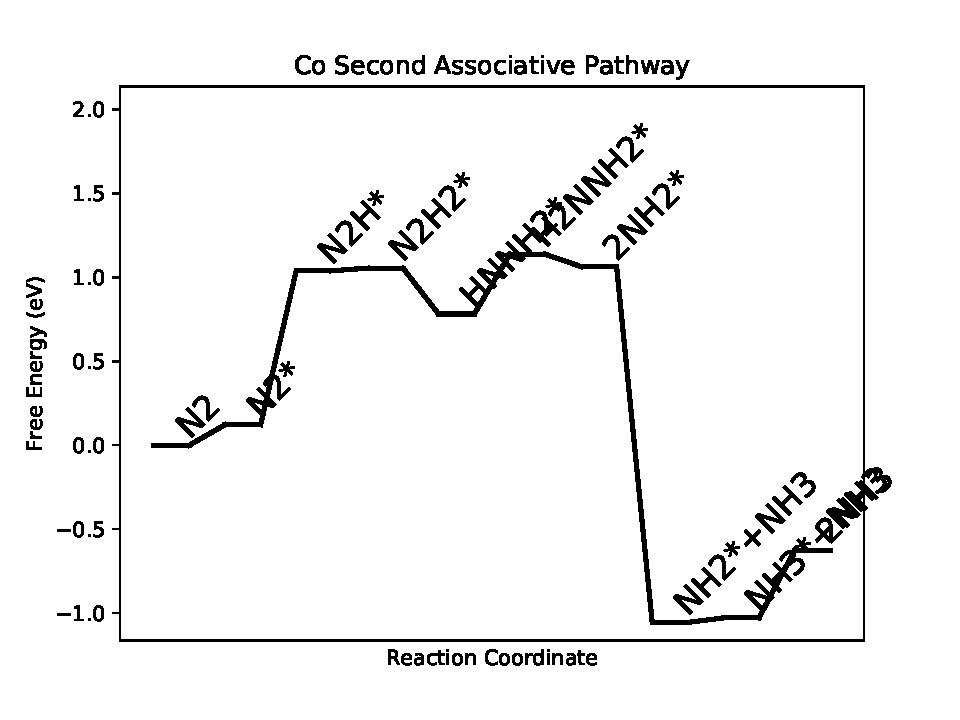
\includegraphics[width=0.8\linewidth]{data/plots/Co_associative_2.pdf}
\end{figure}

\begin{figure}
\centering
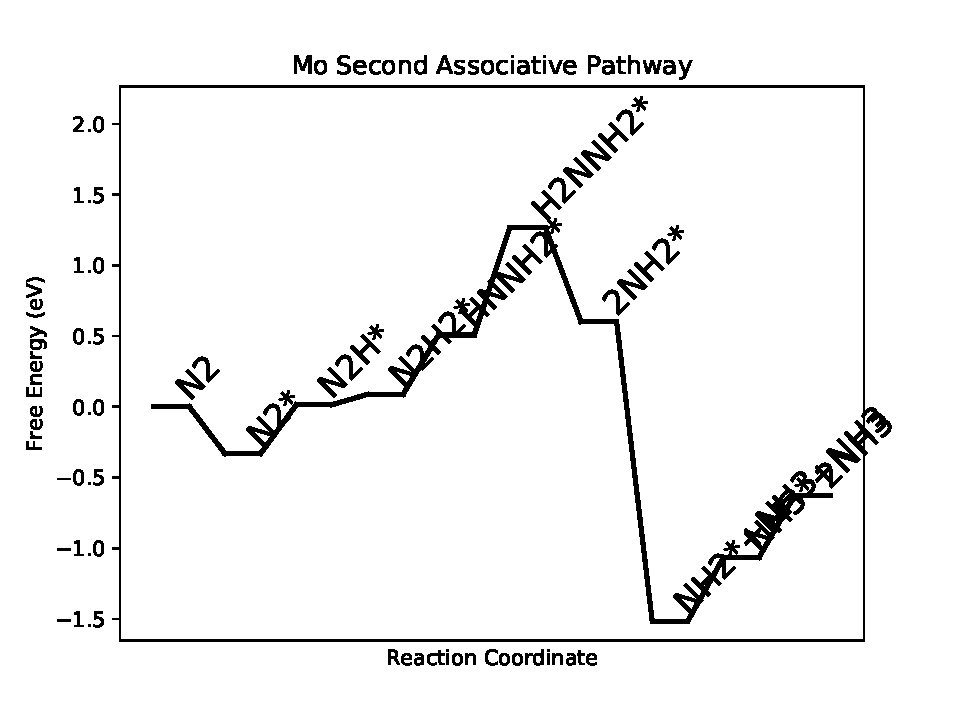
\includegraphics[width=0.8\linewidth]{data/plots/Mo_associative_2.pdf}
\end{figure}

\begin{figure}
\centering
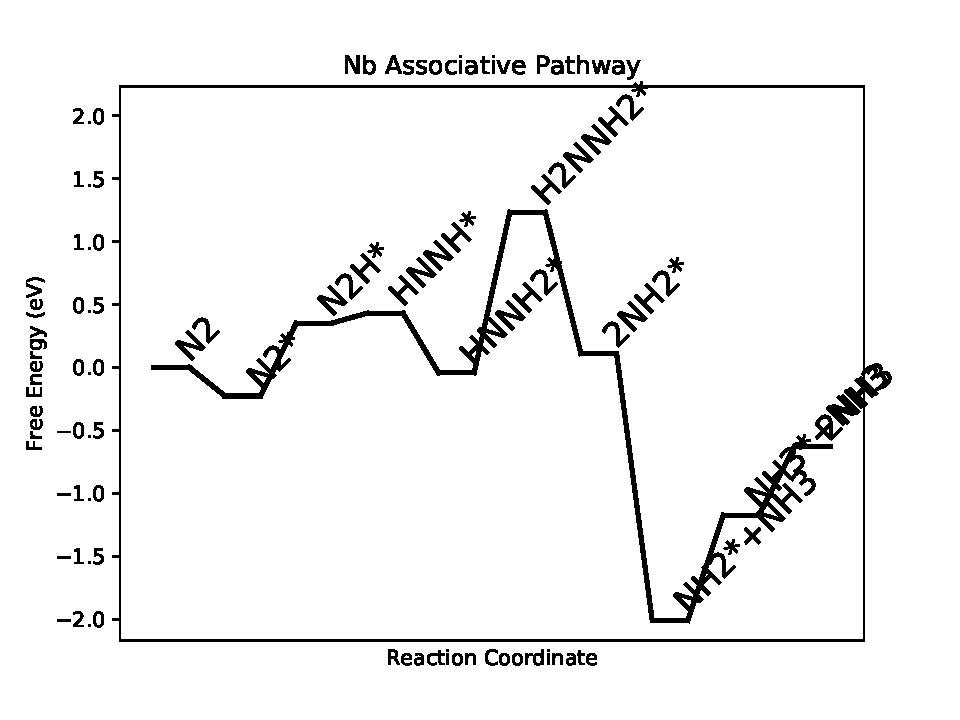
\includegraphics[width=0.8\linewidth]{data/plots/Nb_associative.pdf}
\end{figure}

\begin{figure}
\centering
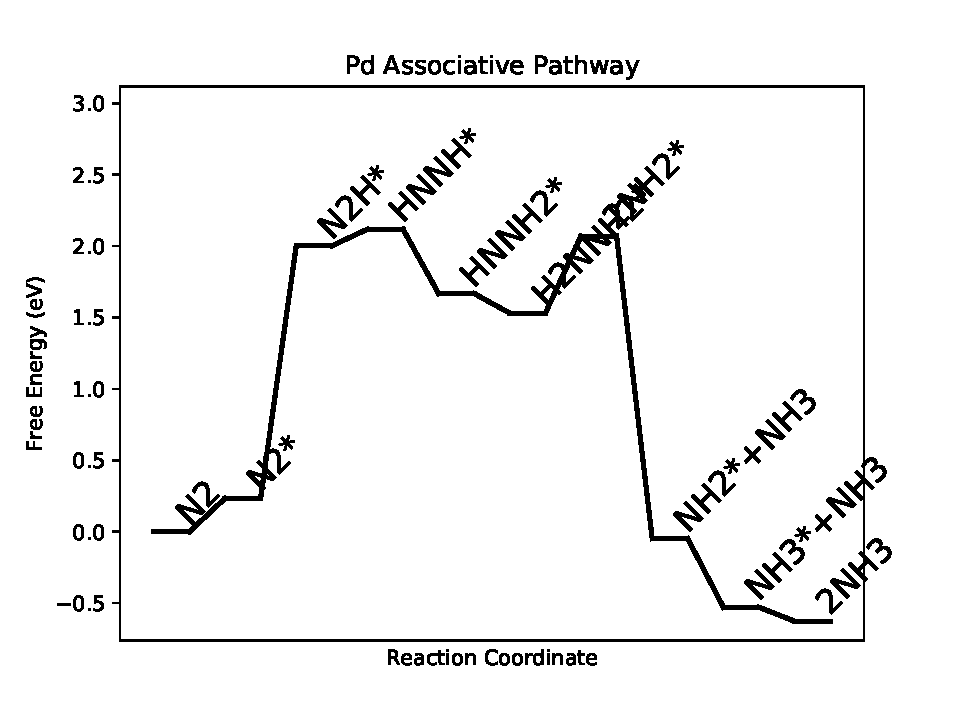
\includegraphics[width=0.8\linewidth]{data/plots/Pd_associative.pdf}
\end{figure}

\begin{figure}
\centering
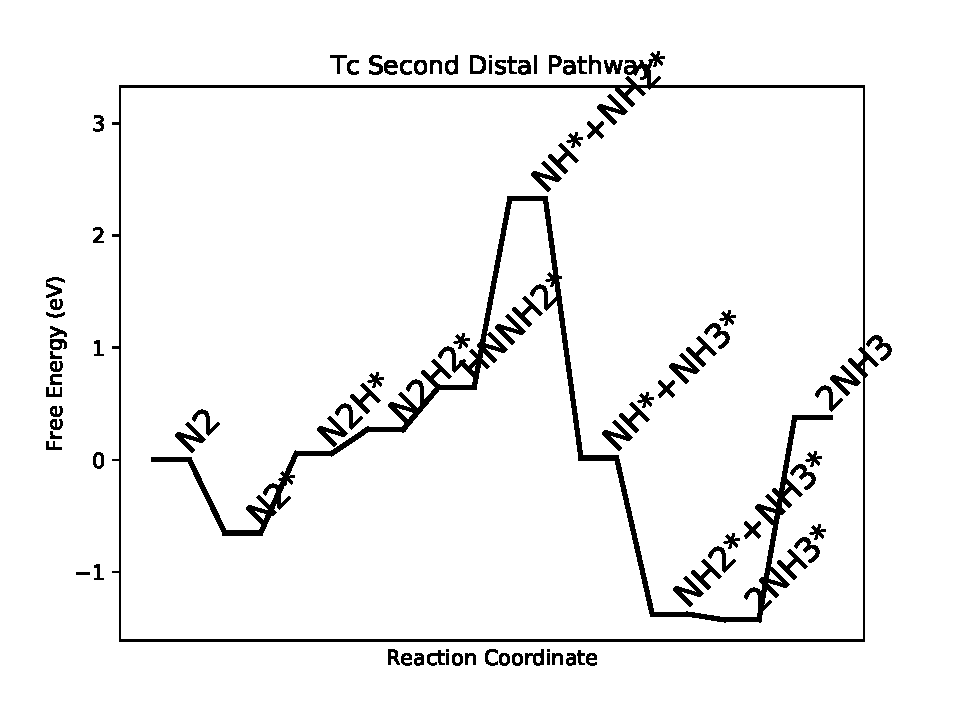
\includegraphics[width=0.8\linewidth]{data/plots/Tc_distal_2.pdf}
\end{figure}

\begin{figure}
\centering
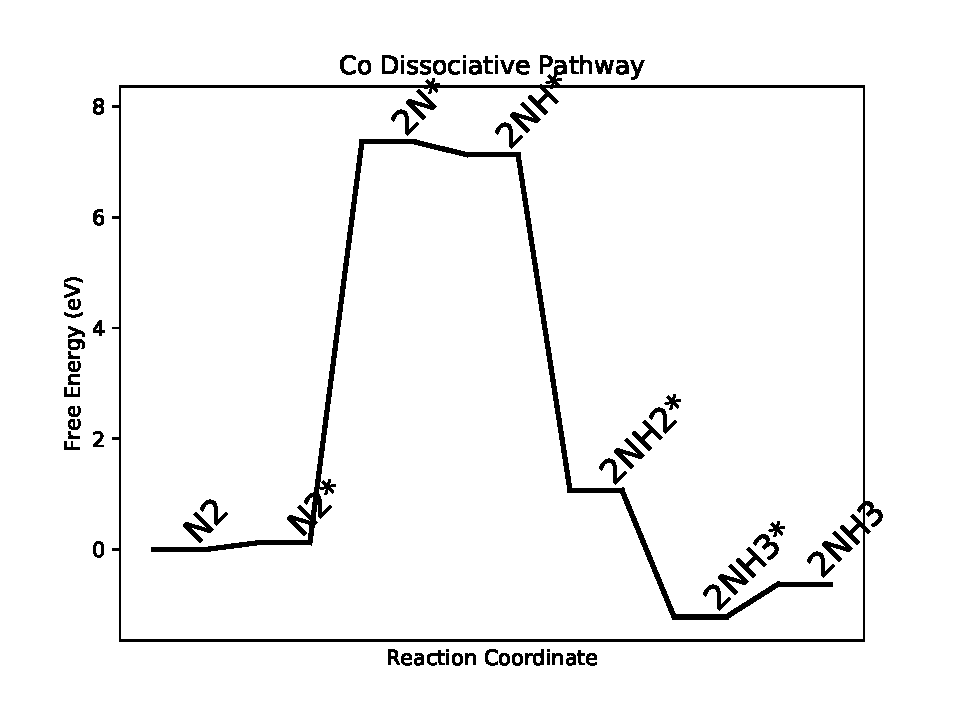
\includegraphics[width=0.8\linewidth]{data/plots/Co_dissociative.pdf}
\end{figure}

\begin{figure}
\centering
\includegraphics[width=0.8\linewidth]{data/plots/Mo_associative.pdf}
\end{figure}

\begin{figure}
\centering
\includegraphics[width=0.8\linewidth]{data/plots/Pd_distal_2.pdf}
\end{figure}

\begin{figure}
\centering
\includegraphics[width=0.8\linewidth]{data/plots/Nb_associative_2.pdf}
\end{figure}

\begin{figure}
\centering
\includegraphics[width=0.8\linewidth]{data/plots/W_associative.pdf}
\end{figure}

\begin{figure}
\centering
\includegraphics[width=0.8\linewidth]{data/plots/Ag_dissociative.pdf}
\end{figure}

\begin{figure}
\centering
\includegraphics[width=0.8\linewidth]{data/plots/Y_dissociative.pdf}
\end{figure}

\begin{figure}
\centering
\includegraphics[width=0.8\linewidth]{data/plots/Nb_dissociative.pdf}
\end{figure}

\begin{figure}
\centering
\includegraphics[width=0.8\linewidth]{data/plots/Sc_distal_1.pdf}
\end{figure}

\begin{figure}
\centering
\includegraphics[width=0.8\linewidth]{data/plots/Nb_distal_2.pdf}
\end{figure}

\begin{figure}
\centering
\includegraphics[width=0.8\linewidth]{data/plots/W_distal_2.pdf}
\end{figure}

\begin{figure}
\centering
\includegraphics[width=0.8\linewidth]{data/plots/Ta_dissociative.pdf}
\end{figure}

\begin{figure}
\centering
\includegraphics[width=0.8\linewidth]{data/plots/Tc_distal_1.pdf}
\end{figure}

\begin{figure}
\centering
\includegraphics[width=0.8\linewidth]{data/plots/Re_distal_1.pdf}
\end{figure}

\begin{figure}
\centering
\includegraphics[width=0.8\linewidth]{data/plots/Ti_associative_2.pdf}
\end{figure}

\begin{figure}
\centering
\includegraphics[width=0.8\linewidth]{data/plots/Ru_distal_1.pdf}
\end{figure}

\begin{figure}
\centering
\includegraphics[width=0.8\linewidth]{data/plots/V_associative.pdf}
\end{figure}

\begin{figure}
\centering
\includegraphics[width=0.8\linewidth]{data/plots/Ni_associative.pdf}
\end{figure}

\begin{figure}
\centering
\includegraphics[width=0.8\linewidth]{data/plots/Hf_associative_2.pdf}
\end{figure}

\begin{figure}
\centering
\includegraphics[width=0.8\linewidth]{data/plots/Re_associative_2.pdf}
\end{figure}

\begin{figure}
\centering
\includegraphics[width=0.8\linewidth]{data/plots/Ir_associative_2.pdf}
\end{figure}

\begin{figure}
\centering
\includegraphics[width=0.8\linewidth]{data/plots/Ag_associative_2.pdf}
\end{figure}

\begin{figure}
\centering
\includegraphics[width=0.8\linewidth]{data/plots/Hf_distal_2.pdf}
\end{figure}

\begin{figure}
\centering
\includegraphics[width=0.8\linewidth]{data/plots/Re_distal_2.pdf}
\end{figure}

\begin{figure}
\centering
\includegraphics[width=0.8\linewidth]{data/plots/Sc_associative.pdf}
\end{figure}

\begin{figure}
\centering
\includegraphics[width=0.8\linewidth]{data/plots/Ti_distal_2.pdf}
\end{figure}

\begin{figure}
\centering
\includegraphics[width=0.8\linewidth]{data/plots/Mo_dissociative.pdf}
\end{figure}

\begin{figure}
\centering
\includegraphics[width=0.8\linewidth]{data/plots/Zr_dissociative.pdf}
\end{figure}

\begin{figure}
\centering
\includegraphics[width=0.8\linewidth]{data/plots/Ru_associative.pdf}
\end{figure}

\begin{figure}
\centering
\includegraphics[width=0.8\linewidth]{data/plots/Ag_distal_1.pdf}
\end{figure}

\begin{figure}
\centering
\includegraphics[width=0.8\linewidth]{data/plots/Os_associative.pdf}
\end{figure}

\begin{figure}
\centering
\includegraphics[width=0.8\linewidth]{data/plots/Ag_associative.pdf}
\end{figure}

\begin{figure}
\centering
\includegraphics[width=0.8\linewidth]{data/plots/Co_distal_2.pdf}
\end{figure}

\begin{figure}
\centering
\includegraphics[width=0.8\linewidth]{data/plots/Ta_distal_1.pdf}
\end{figure}

\begin{figure}
\centering
\includegraphics[width=0.8\linewidth]{data/plots/Zr_distal_2.pdf}
\end{figure}

\begin{figure}
\centering
\includegraphics[width=0.8\linewidth]{data/plots/Ta_associative.pdf}
\end{figure}

\begin{figure}
\centering
\includegraphics[width=0.8\linewidth]{data/plots/Pt_distal_1.pdf}
\end{figure}

\begin{figure}
\centering
\includegraphics[width=0.8\linewidth]{data/plots/Cu_associative.pdf}
\end{figure}

\begin{figure}
\centering
\includegraphics[width=0.8\linewidth]{data/plots/Pd_associative_2.pdf}
\end{figure}

\begin{figure}
\centering
\includegraphics[width=0.8\linewidth]{data/plots/Pd_dissociative.pdf}
\end{figure}

\begin{figure}
\centering
\includegraphics[width=0.8\linewidth]{data/plots/Co_associative.pdf}
\end{figure}

\begin{figure}
\centering
\includegraphics[width=0.8\linewidth]{data/plots/V_distal_1.pdf}
\end{figure}

\begin{figure}
\centering
\includegraphics[width=0.8\linewidth]{data/plots/Ti_dissociative.pdf}
\end{figure}

\begin{figure}
\centering
\includegraphics[width=0.8\linewidth]{data/plots/Mo_distal_2.pdf}
\end{figure}

\begin{figure}
\centering
\includegraphics[width=0.8\linewidth]{data/plots/Sc_distal_2.pdf}
\end{figure}

\begin{figure}
\centering
\includegraphics[width=0.8\linewidth]{data/plots/Zr_associative_2.pdf}
\end{figure}

\begin{figure}
\centering
\includegraphics[width=0.8\linewidth]{data/plots/Zr_associative.pdf}
\end{figure}

\begin{figure}
\centering
\includegraphics[width=0.8\linewidth]{data/plots/Os_distal_1.pdf}
\end{figure}

\begin{figure}
\centering
\includegraphics[width=0.8\linewidth]{data/plots/Ti_distal_1.pdf}
\end{figure}

\begin{figure}
\centering
\includegraphics[width=0.8\linewidth]{data/plots/Hf_dissociative.pdf}
\end{figure}

\begin{figure}
\centering
\includegraphics[width=0.8\linewidth]{data/plots/W_associative_2.pdf}
\end{figure}

\begin{figure}
\centering
\includegraphics[width=0.8\linewidth]{data/plots/Zr_distal_1.pdf}
\end{figure}

\begin{figure}
\centering
\includegraphics[width=0.8\linewidth]{data/plots/Hf_distal_1.pdf}
\end{figure}

